\documentclass[]{report}

\usepackage[a4paper, total={6in, 8in}]{geometry}
\usepackage{amsfonts}
\usepackage{amsmath}
\usepackage{amsthm}
\usepackage{hyperref}
\usepackage{tikz}
\usepackage{graphicx}
\usepackage{float}
\usepackage[boxruled,linesnumbered]{algorithm2e}
\usepackage{multirow}
\usepackage{cleveref}
\usepackage{wrapfig}
\usepackage{caption}
\usepackage{subcaption}
\usepackage{enumitem}
\usepackage{adjustbox}
\usepackage{pifont}

\theoremstyle{plain}
\newtheorem{theorem}{Theorem}[section]
\newtheorem{lemma}[theorem]{Lemma}
\newtheorem{proposition}[theorem]{Proposition}
\newtheorem*{corollary}{Corollary}

\theoremstyle{definition}
\newtheorem{definition}{Definition}[section]
\newtheorem{conjecture}{Conjecture}[section]
\newtheorem{example}{Example}[section]

\theoremstyle{remark}
\newtheorem*{remark}{Remark}
\newtheorem*{note}{Note}

\crefname{algocf}{alg.}{algs.}
\Crefname{algocf}{Algorithm}{Algorithms}

\theoremstyle{plain}
\newtheorem{assumption}{Assumption}

%Title
\title{Some Security Considerations over Contiki-based Sensor Network}
%Authors
\author{Yan Yan}
\date{\today}



\begin{document}

\maketitle

\tableofcontents

%Body
%%\chapter{Some Chapter}

\section{Some Section}

Contents\cite{SomeCitation}...

\section{Introduction}
Applications for the Internet of Things (IoT) flourish, leaving a great desire for not only energy efficient, cheap devices, but also for devices that support basic cryptographic functionality such as confidentiality and/or authenticity. Popular algorithms for confidentiality are e.g. the Advanced Encryption Standard\cite{AES}, and the Elliptic Curve Digital Signature Algorithm\cite{ECDSA}, which, when used in conjunction, enable to establish secure end-to-end channels via e.g. Datagram TLS\cite{DTLS}. 

However whilst AES is a secure block cipher, one might require randomness to turn it into a secure encryption scheme for arbitrary length messages. Somewhat similarly, ECDSA relies on a known-to-be-secure mathematical problem. However, it also requires large and securely generated random numbers. Consequently, when supporting cryptography the secure generation of random numbers is crucial. 

%The prospering IoT applications constantly proposes higher requirements to security where cryptography plays an important role. Among all prerequisite of implementing cryptographic primitives on these IoT devices, a reliable Random Number Generator (RNG) is critical as it is required in most cryptographic algorithms. In practice, a RNG typically involves a Pseudo Random Number Generator (PRNG) seeded by a high entropy physical source.

In 2013, Texas Instruments (TI) launched a new System-on-chip (SoC), the CC2538\cite{CC2538}, featuring secure channels via 802.15.4\cite{802154Standard} support via multiple cryptographic hardware accelerators. Partially because this cryptographic accelerators, projects such as Contiki\cite{Contiki} and OpenWSN\cite{OpenWSN} began to support the CC2538 with enthusiasm. As of writing this paper, the chip features in the suggested list for Zigbee and 6LoWPAN solution on TI's website\cite{ZigbeeProducts}\cite{6LowPANProducts}.

However, despite all the cryptographic hardware support, the CC2538 does not have a RNG dedicated for cryptographic applications; instead, the user manual suggests to use a 16 bit Linear Feedback Shift Register (LFSR) as a PRNG where the seed is generated by the Radio Frequency (RF) module sampling from the radio noise. Whilst the user guide at no point suggests that this method should be used in conjunction with cryptographic algorithms, developers have little choice in the absence of alternatives. Also, in the absence of published attacks, there is often a temptation to ignore warnings such as in \cite{SmartMeterBlog}. 

\subsection{Our Contribution}
We show in this study that this choice proves catastrophic for cryptographic applications, not only because the in-built PRNG has only 16 bit entropy which can be easily predicted, but also because we are able to practically demonstrate how to use radio jamming to bias the seed obtained from the RF module. Consequently, even if the weak in-built PRNG was replaced by a stronger component, the source for the seed could still be tampered with and thus render the system insecure. All the experimental work in this paper was performed on Contiki OS\cite{Contiki} release version 3.0. 
%The related source code can be accessed at \cite{prngtest}.

Our paper is structured as follows. We begin in \Cref{ContikiDriverIssue} with some Contiki RNG driver issues for CC2538. \Cref{LFSR} revises why using a 16 bit LFSR as PRNG is a bad practice and we show how this design flaw can be exploited to break DTLS in \Cref{BreakDTLS}, before reviewing the problem in \Cref{PRNGReflection}. In \Cref{Seed} we explain how CC2538 samples the radio noise into random seed and then we demonstrate how it can be biased by jamming signals in \Cref{Jamming}. Finally we conclude the paper in \Cref{Conclusion}.

\subsection{Related Work}
The design flaw of using a 16 bit LFSR as PRNG has been reported by \cite{SmartMeterBlog}\cite{CC2530PRNG} on CC2430\cite{CC2430Manual} and CC2530\cite{CC2530Manual} respectively. These chips are the predecessors of CC2538 in the SimpleLink\cite{SimpleLink} series and they all adopted the same RNG design. The blogs reported the flaw and warned that it could easily be exploited to break the Z-Stack library\cite{ZStack} and Smart Energy Profile ECC in many Smart Meter applications. We essentially `rediscovered' that this poor design choice still features in the CC2538 product. However, whilst in previous work the possibility of injecting a jamming signal was contemplated, we are the first to actually examine the technical feasibility of this and to demonstrate a working attack.


\subsection{Contiki Driver Issues}\label{ContikiDriverIssue}
We made extensive use of Contiki in our research and fixed (and reported) some coding issues in their RNG driver (release-3.0). These were, the reading out of the LFSR without ready check, a lack of validity check when reading random seed bits from the RF module, and a bug that drops the Most Significant Bit (MSB) and leaves the Least Significant Bit (LSB) to be constantly zero in the seed.  We modified the code and fixed these issues in our experiments. 

Another issue in the driver is that the CC2538 User's Guide\cite{CC2538Manual} suggests only to use the lower byte (8 bits) as a random number but the driver actually used 16 bits in the LFSR. However, this coding mistake does not affect our result, as will be explained in  later sections.
\chapter{Preliminaries:\\ Building Blocks of WSN} \label{Chp: Building Blocks}

In this chapter, we introduce the building blocks of a WSN using OSI model\cite{OSI}.

The data channel in OSI model is descried as a set of protocols stacked layer by layer from the Physical Layer at the bottom to the Application Layer at the top (\Cref{fig: OSI model}). Ideally, lower layer protocols provide an universal  interface to upper layer protocols; thus providing flexibility to protocol choice in different scenarios as well as interoperability between nodes with different lower level structures.

\begin{figure*}[h!]
	\centering
	{
		\includegraphics[width=0.4\textwidth,]{fig/Osi-model-jb.png}
	}
	\caption{OSI model} \label{fig: OSI model}
\end{figure*}

\Cref{fig: OSI channel} demonstrates a typical data transmission in OSI modelled network. The application data is encapsulated by the sender from top to the bottom, with each encapsulation adds additional metadata, namely protocol headers, to the data. The receiver unwinds the process and reads out the data.

\begin{figure*}[h!]
	\centering
	{
		\includegraphics[width=0.6\textwidth,]{fig/osi-model.png}
	}
	\caption{Data Transfer in OSI model} \label{fig: OSI channel}
\end{figure*}

However, in real world scenarios the boundaries between the top three layers are usually ambiguous; many context, including this report, simply refers them all together as Application Layer. In most scenarios the application only needs the Transport Layer interfaces and anything beneath is transparent.

A selection of protocols at each layer is called a protocol suite, or a protocol stack. 8 bits is called an OCTET in network terminology but for readability in general computer science we use BYTE to represent the unit of 8 bits.

Protocols from Physical Layer to Transport Layer are implemented by hardware or kernel. Since most IoT devices are extremely resource constrained; thus it is hard to directly transplant the widely used TCP/IP protocol suite to WSNs. Instead, different protocols and operating systems are specifically designed for WSN applications. Contiki\cite{Contiki} is a highly customisable IoT system with 6LoWPAN\cite{rfc4919} support and can run on many recent IoT hardware, OpenWSN\cite{OpenWSN} is also a popular IoT system that has well integrated 6LoWPAN with CoAP\cite{rfc7252} and FreeRTOS\cite{FreeRTOS} is optimised for real time applications, etc. There are many other IoT systems and protocols that we do not list here. In this research, we build our experimental WSN over Contiki with 6LoWPAN due to their popularity in academic and industry.

Following in \Cref{Chp: Building Blocks} we introduce the building blocks of our experimental WSN from the bottom to the top in OSI model.

\section{Physical Layer}
Physical Layer protocols (or standards) specify the hardware requirements. They basically defines how a bit is transmitted over a physical medium.

WSN features, as can be seen by its name, wireless connectivity. 802.15.4\cite{802154} standard is supported in many recent WSN devices. The  802.15.4 Physical Layer specification, 802.15.4 PHY, is crafted to be suitable for embedded wireless devices emphasising low energy, low cost and low speed. Bluetooth Low Energy\cite{BLE}, BLE, is another candidate for WSN with similar features. \cite{802154BLE} provides a performance analysis of 802.15.4 and BLE.

\Cref{Fig: 802.15.4 PHY Frame} shows the constitution of a Physical Layer frame. A frame is a bit string transmitted sequentially from the left in the figure to the right. We use the same representations for the rest in \Cref{Chp: Building Blocks}.

\begin{table}[h!]
	\centering
	\begin{tabular}{|c|c|c|c|c|}
		\hline
		Preamble & SFD & MAC Frame Length & Reserved & MAC Frame\\ \hline
	\end{tabular}
	\caption{802.15.4 PHY Frame}
	\label{Fig: 802.15.4 PHY Frame}
\end{table}

We omit the further details of 802.15.4 PHY standard as they strongly relate to hardware details which is beyond the scope of this report. We give only a brief explanation of the contents in the frame.

\textbf{Preamble} is a flag used for hardware synchronisation. \textbf{Start Frame Delimiter}, SFD, is a constantly 0xE5 for 802.15.4 frames which marks the begin of data in this frame. \textbf{MAC Frame Length} is a value of 0 to 127 indicating the number of bytes in the following \textbf{MAC Frame}, which we explain in \Cref{Sec: Data Link Layer}.

Our experimental WSN is built on TelosB\cite{TelosB} and CC2538\cite{CC2538}. Wismote\cite{Wismote} is also used in Cooja simulations.

\section{Data Link Layer} \label{Sec: Data Link Layer}
Data Link Layer protocols manages the Physical Layer channel. In case of WSN, this is effectively Radio Frequency, RF. Data Link protocols are strongly related to physical features of underlining devices. 

Data Link Layer is  also referred as Media Access Control, MAC, Layer for convenience. A MAC Frame is the atomic data transferring unit in this layer. MAC Layer protocols define data transmission between physically connected devices, i.e. single hop communication. Packet forward is defined in upper layer protocols.

In case of WSN, a MAC Frame is always broadcasted to the sender’s neighbour due to the physical nature of RF. To avoid interference, MAC protocols adopts  techniques such as CSMA/CA \cite{802154} or TSCH\cite{TSCH} to solve the problem of how MAC Frames should be sent. Further more, other techniques like ContikiMAC\cite{ContikiMAC} proposes a sub Radio Duty Cycle, RDC, Layer protocol that aims to improve the energy efficiency of RF.

As of this research, we are more focused on the contents in a MAC Frame defined by 802.15.4 MAC Layer specification\cite{802154}, 802.15.4 MAC.

\subsection{802.15.4 MAC} \label{Subsec: 802.15.4 MAC}
802.15.4 MAC defined four types of MAC Frames.
\begin{description}[style=nextline]
	\item[\textbf{Beacon}] 
	Beacon frame is broadcasted to physically organise the network.
	\item[\textbf{Command}] 
	Command frame is used for data channel maintenance.
	\item[\textbf{Data}] 
	Data frame carries data from upper layer protocols.
	\item[\textbf{ACK}] 
	ACK frame only optionally sent in response when requested by other frames to notify the sender that the frame is received. Some protocols use ACK frames, e.g. ContikiMAC uses it to inform the sender that the frame is received and hence terminates the resending process of sender.
\end{description}

We are particularly interested in Data frames as they are most relevant to application data. \Cref{Fig: 802154 Data Frame} describes its format.

\begin{figure*}[h!]
	\centering
	\begin{tabular}{|c|c|c|c|c|}
		\multicolumn{3}{c}{\textit{MAC Header}}                           & \multicolumn{1}{c}{\textit{MAC Payload}} & \multicolumn{1}{c}{\textit{MAC Footer}}     \\ \hline
		2 (bytes)     & 1                    & 4 to 20              & *           & 2              \\ \hline
		Frame Control & Sequence Number & Address Information & Data        & Frame Checksum \\ \hline
	\end{tabular}
	\caption{802.15.4 Data Frame}
	\label{Fig: 802154 Data Frame}
\end{figure*}

\begin{description}[style=nextline]
	\item[\textbf{Frame Control}]
	This field contains the bit flags instructing how the receiver should interpret this frame, such as the type of frame, with ACK and security options on or not, and format of addresses, etc. When the security option is enabled, additional field will be added to the frame. We explain the security enabled frame later in \Cref{Subsec: 802154 Sec}. The full details of flags is defined by \cite{802154}.
	
	\item[\textbf{Sequence Number}]
	The sequence number is increased by one for each MAC Frame sent and wraps to 0 when reached maximum. The sequence number is mostly used to match ACKs when requested.
	
	\item[\textbf{Address Information}]
	This field contains source and destination MAC address of this frame. Their length are variable and is specified in Frame Control. Simply speaking, longer addresses are for larger networks and shorter for smaller ones. MAC address is derived from hardware and should be unique but configurable during runtime. As stated earlier, a MAC Frame is always received by all neighbours of the sender; therefore the receiver who does not match the destination will immediately drop the frame without processing it to upper layer.
	
	\item[\textbf{Data}]
	This is the MAC Layer data containing upper layer protocol headers and application data.
	
	\item[\textbf{Frame Checksum}]
	The checksum is used to check and correct the error induced by physical channel.
\end{description}

Frame Control, Sequence Number and Address Information together are called MAC Header. Data is therefore called MAC Payload respectively. 

As specified in 802.15.4 PHY, Maximum Transmission Unit, MTU, required by 802.15.4 MAC Frame is 127 bytes including the MAC header and footer. In other words, 802.15.4 compatible hardware are guaranteed to send frames up to 127 bytes but frames exceeding this value might be silently discarded. Since MAC Header and Footer consumes 25 bytes in a Data frame, there is actually 102 bytes left for MAC Payload.

Setting the security flag in Frame Control enables 802.15.4 Security and adds additional fields into the MAC header, which we describe in \Cref{Subsec: 802154 Sec}.

\subsection{802.15.4 Security} \label{Subsec: 802154 Sec}
802.15.4 Security is based on Authenticated Encryption with Associated Data, AEAD, with AES-128 being the underlining block cipher. Specifically, it provides encryption for MAC Payload and authenticity for the whole MAC Frame.

The format of a 802.15.4 Data frame with security option set is described in \Cref{Fig: 802154 sec frame}.

\begin{figure*}[h!]
	\centering
	\begin{tabular}{|c|c|c|c|c|c|c|}
		\multicolumn{4}{c}{\textit{MAC Header}}                                                             & \multicolumn{2}{c}{\textit{MAC Payload}} & \multicolumn{1}{c}{\textit{MAC Footer}}     \\ \hline
		\multicolumn{3}{|c|}{\multirow{2}{*}{As MAC Header in \Cref{Fig: 802154 Data Frame}}} & 0 to 14 (bytes)                    & *             & 0/4/8/16         & 2              \\ \cline{4-7} 
		\multicolumn{3}{|c|}{}                                           & Auxiliary Security Header & Data          & MIC              & Frame Checksum \\ \hline
	\end{tabular}
	\caption{802.15.4 Frame with security option enabled} \label{Fig: 802154 sec frame}
\end{figure*}

The Auxiliary Security Header controls the security primitive and materials in 802.15.4 Security as shown in \Cref{Fig: Auxiliary Security Header of 802.15.4 Security}.

\begin{figure*}[h!]
	\center
	\begin{tabular}{|c|c|c|}
	\hline
	\multicolumn{3}{|c|}{Auxililary Security Header} \\ \hline
	3 bits          & 4 byte         & *             \\ \hline
	Security Level  & Frame Counter  & Key Strategy  \\ \hline
	\end{tabular}
	\caption{Auxiliary Security Header of 802.15.4 Security}
	\label{Fig: Auxiliary Security Header of 802.15.4 Security}
\end{figure*}

\begin{description}[style=nextline]
	\item[\textbf{Security Level}]
	Security Level is represented by the first 3 bits in Auxiliary Security Header. The highest bit enables encryption and lower two bits controls the length of Message Integrity Code, MIC, which is equivalent to Message Authenticate Code in cryptographic terms.  MIC of $0$ length indicates no authentication. Particularly, the security level can be configured to be:
	\begin{itemize}
		\item Encryption only. Only MAC Payload is encrypted in CTR mode.
		\item Authentication only. A CBC-MIC\footnote{Equivalent to CBC-MAC in cryptographic term.} computed on the whole frame is attached to the end of Data. Data is transmitted in plaintext. Length of the MIC can be either 32, 64 or 128 bits based on the lower two bits of Security Level.
		\item Encryption and authentication. The whole frame is processed in CCM*\cite{802154} mode. MAC Header is the associated data and MAC Payload the plaintext. The asterisk symbol requires that the nonce, or IV, must can be decoded to uniquely determine the exact format of output ciphertext. Length of the MIC can be either 32, 64 or 128 bits based on the lower two bits of Security Level.
	\end{itemize}
	\item[\textbf{Frame Counter}]
	4 bytes of Auxiliary Security Header is occupied by Frame Counter which increases by one for each frame sent. It constitutes part of the nonce in CCM* mode and is also used for replay detection.
	\item[\textbf{Key Strategy}]
	Key Strategy instructs which key to be used for this frame. The keys are presumed to be pre-shared in PAN\footnote{Personal Area Network} Information Base, PIB, which is a database containing information that is shared among the network. Keys are managed by groups and indexes within a group. The definition of groups depends on upper layer applications. The length of Key Strategy is variable.
\end{description}

More details of Auxiliary Security Header is defined by \cite{802154}.

Access Control List, ACL, is a data structure used to manage the keys during runtime. Each entry of ACL is paired with another node.  An ACL entry contains the following elements:
\begin{description}[style=nextline]
	\item[\textbf{Address}]
	The remote address, used as an identifier of ACL entry.
	\item[\textbf{Security Suite}]
	Effectively the Security Level associated to the remote address.
	\item[\textbf{Key}]
	The paired cryptographic key associated to the remote address.
	\item[\textbf{Last Initial Vector}]
	Nonce used for the last outgoing frame. Used to deduce next nonce to use.
	\item[\textbf{Replay Counter}]
	Nonce received for the last incoming frame. Used when replay protection is on.
\end{description}

One thing to be noticed is that neither Key Strategy nor ACL is implemented on our platform. We give more details about key management of 802.15.4 Security in Contiki implementation in \Cref{Subsec: 802.15.4 Security Implementation in Contiki}.

\subsection{Nonce of CCM* in 802.15.4 Security}
As stated earlier in \Cref{Subsec: 802154 Sec}, CCM* requires that the format of ciphertext can be uniquely deduced from the nonce. \Cref{Fig: CCM nonce} describes the nonce used for encryption.

\begin{figure*}[h!]
	\centering
	\begin{tabular}{|c|c|c|c|c|}
		\hline 
		1 (bytes) & 8              & 4             & 1              & 2             \\ \hline
		Flag      & Source Address & Frame Counter & Security Level & Block Counter \\ \hline
	\end{tabular}
	\caption{CCM* nonce for encryption}
	\label{Fig: CCM nonce}
\end{figure*}

\begin{description}[style=nextline]
	\item[\textbf{Flag}]
	 Deduced by MTU. In case of 802.15.4, it is constantly 0x02.
	\item[\textbf{Source Address}]
	Address of sender. Addresses less than 8 bytes will be extended.
	\item[\textbf{Frame Counter}]
	Directly mapped from Frame Counter in Auxiliary Security Header.
	\item[\textbf{Security Level}]
	Directly mapped from Security Level in Auxiliary Security Header with the highest bit set to $0$. Security Level solely determines the format of ciphertext.
	\item[\textbf{Block Counter}]
	Index of data blocks in MAC payload, with the first block being 0 and increases by one for each block. The block length is 128 bits since AES-128 is the underlining block cipher.
\end{description}

802.15.4 Security could either be implemented by hardware and/or software. Some platform may not support the security option, or only a sub set. We describe the 802.15.4 Security implementation on Contiki in \Cref{Subsec: 802.15.4 Security Implementation in Contiki}.

\subsection{802.15.4 Security Implementation in Contiki} \label{Subsec: 802.15.4 Security Implementation in Contiki}
noncoresec\cite{noncoresec} is the 802.15.4 Security implementation in Contiki. It is a reduced implementation of 802.15.4 Security which supports only a network shared key hard coded into the kernel code.

\subsection{Sub Layer: RDC Layer}

In practical, the radio transceiver turned out to be the most energy consuming part in a sensor node. Further more, listening to data consumes more energy than sending. Therefore an improvement of energy efficiency is to switch off the transceiver for most of the time and only turn it on when there is data on air. The Radio Duty Cycle, RDC, Sub Layer is therefore defined as part of MAC Layer which controls the behaviour of radio transceiver.

There are two RDC protocols implemented in our platform.

\begin{itemize}
\item \textbf{nullrdc}. There is no RDC protocol. The transceiver is always kept on.
\item \textbf{ContikiMAC\cite{ContikiMAC}}. The transceiver is kept off for most of the time and only wakes up for a short period. If data transmission is detected during the wake-up period, the receiver keeps the transceiver on until the frame is received and informs the sender with an ACK. On the other hand, the sender continuously retransmits the frame until an ACK is received or timeout.
\end{itemize}

Time-Slotted Channel Hopping\cite{TSCH}, TSCH, is another RDC protocol that is adopted by OpenWSN. We omit its further detail as it is not yet implemented on our platform.

\section{Network Layer} \label{Sec: Network Layer}
The MAC Layer protocols defined the data transmission over directly linked nodes. However, real world applications are usually deployed in a wider range that physically cannot be covered by only direct connections, such as smart city applications. The solution is to build a logical connection that allows the data to be forwarded by intermediate nodes until it reaches the destination. Such logical connection is called a multi hop connection with respect to directly connected single hop connection. As a result, arbitrary nodes can connect to each others and hence forms a network.

Network Layer protocols aim at the routing and addressing problems. The transmission unit in Network Layer is called a packet. The headers and payload constitutes the MAC Payload as in \Cref{Fig: 802154 Data Frame}.

There are two typical types of network in WSN applications:
\begin{description}[style=nextline]
	\item[\textbf{Star Network}]
	Star network is a type of centralised network as depicted in \Cref{fig: Star Network}. Each node is directly linked to the centre one. 
	\item[\textbf{Mesh Network}]
	Mesh network has a decentralised structure as depicted in \Cref{fig: Mesh Network}. Comparing to star network, packets are routed in a mesh network.
\end{description}
%CONTINUE FROM HERE 20160218
\begin{figure*}
	\centering
	\begin{subfigure}[b]{0.5\textwidth}
		{
			\includegraphics[width=0.5\textwidth,]{fig/StarNetwork.png}
		}
		\subcaption{Star Network} \label{fig: Star Network}
	\end{subfigure}
	\begin{subfigure}[b]{0.5\textwidth}
		{
			\includegraphics[width=0.5\textwidth,]{fig/NetworkTopology-Mesh.png}
		}
		\subcaption{Mesh Network} \label{fig: Mesh Network}
	\end{subfigure}
	\caption{Network Topologies} \label{fig: Network topologies}
\end{figure*}

%Some network are built with a hybrid approach of star network and mesh network, e.g. the Cluster Tree Network of Zigbee\cite{Zigbee} as showed in \Cref{fig: ZigBee Topologies}.
%
%\begin{figure*}[h!]
%	\centering
%	{
%		\includegraphics[width=0.7\textwidth,]{fig/ZigBeeTopologies.png}
%	}
%	\caption{Different ZigBee Network Topologies} \label{fig: ZigBee Topologies}
%\end{figure*}

Star network is easier to implement and therefore requires less resources. Mesh network is more complicated but it is more flexible, scalable and robust.

In this research, we build our experimental WSN using 6LoWPAN without loss of generality, as it is supported by most recent WSN systems.



\subsection{6LoWPAN} \label{Subsec: 6LoWPAN}
6LoWPAN is an emerging standard in WSN applications. 6LoWPAN has the following features: 
\begin{itemize}
	\item It is standardised by IETF and is well supported in industry.
	\item Each device is assigned an IPv6 address. This feature provides a great potential of interoperability with other Internet devices, such as a desktop or a smart phone.
	\item As a mesh network, it is flexible, scalable and robust, since the network can dynamically reorganise itself during runtime.
\end{itemize}

Simply speaking , 6LoWPAN packets can be categorised into two classes:
\begin{itemize}
	\item \textbf{IPv6 Data Packets}
	\item \textbf{ICMPv6 Packets}
\end{itemize}
We give a brief explanation of their contents in \Cref{Subsec: IPv6 Data Packets} and \Cref{Subsec: ICMPv6} respectively.

\subsection{6LoWPAN Adaptation Sub Layer} \label{Subsec: 6LoWPAN Adaptation Sub Layer}
A sub layer is defined in 6LoWPAN standard\cite{rfc4944} which adapts IPv6\cite{rfc2460} to constrained environment by header compression. An adaption headers is prepended before the IPv6 header as shown in \Cref{Fig: 6LoWPAN Adaptation Header}. 

\begin{figure*}[h!]
	\centering
	\begin{tabular}{|l|l|l|}
		\hline
		6LoWPAN Adaptation Header & Compressed IPv6 Header & IPv6 Payload \\ \hline
	\end{tabular}
	\caption{6LoWPAN Adaptation Header}
\label{Fig: 6LoWPAN Adaptation Header}
\end{figure*}

The compression is basically done by:
\begin{itemize}
	\item Optimised encoding. Take the Hop Limit, HLIM or TTL (Time To Live), field for example, the frequently used values, 1, 64 and 255, are represented in 2 bits as 01b, 10b and 11b respectively, saving 6 bits from its original 1 byte field.
	\item Shortened addresses. Since 6LoWPAN has usually less devices than a normal IPv6 network, the unused higher bits can be omitted. The shortened addresses can be extended on need.
\end{itemize}

The header compression is lossless; thus an equivalent IPv6 header can always be reconstructed. We omit further details of compression as it is beyond the scope of this research but the scheme is defined in \cite{rfc6282}.

In addition to header compression information, 6LoWPAN Adaptation sub layer may optionally contains packet fragmentation information and routing information. We omit further details of them as they are beyond the scope of this research. Details are defined in \cite{rfc4944}.

\subsection{IPv6 Data Packets} \label{Subsec: IPv6 Data Packets}

IPv6 Data Packets carry the IPv6 Payload. In 6LoWPAN, the IPv6 header is compressed as described in \Cref{Subsec: 6LoWPAN Adaptation Sub Layer}. In this section, we use a standard IPv6 header in description instead for convenience, as it is bijective to its compressed format.

IPv6 packet is defined in \cite{rfc2460}. We show its basic format in \Cref{Fig: Basic IPv6 Packet Format}. Length information are omitted in the figure as they are inconsistent when compressed.

\begin{figure*}[h!]
\center
	\begin{tabular}{l|c|c|c|c|c|c|}
	\cline{2-7}
	\multirow{2}{*}{\textit{IP Header}} & Version & Traffic Class & Flow Label & Payload Length & Next Header & Hop Limit \\ \cline{2-7} 
	                                & \multicolumn{3}{c|}{Source Address}  & \multicolumn{3}{c|}{Destination Address} \\ \cline{2-7} 
	\textit{IP Payload}                 & \multicolumn{6}{c|}{Payload}                                                    \\ \cline{2-7} 
	\end{tabular}
	\caption{Basic IPv6 Packet Format} \label{Fig: Basic IPv6 Packet Format}
\end{figure*}

\begin{description}[style=nextline]
	\item[\textbf{Version}]
	In 6LoWPAN this is constant 0x6.
	\item[\textbf{Traffic Class}]
	This field is default by 0 and may be set by an upper layer application as a hint of packet. A router can act accordingly to this field, such as adjusting the priority of packet, or even modify this value upon forward. The support for values other than $0$ is optional.
	\item[\textbf{Flow Label}]
	This field is intended to label a logical data path at Network Layer. The IPv6 standard\cite{rfc2460} states  it should ``be used by a source to label sequences of packets for which it requests special handling by the IPv6 routers, such as non-default quality of service or `real-time` service``. Support to this field is optional.
	\item[\textbf{Payload Length}]
	This field specifies the length of Payload.
	\item[\textbf{Next Header}]
	This field specifies the Transportation Layer protocol to be used. In WSN applications this is usually UDP. We introduce more details in \Cref{Sec: Transport Layer}.
	\item[\textbf{Hop Limit}]
	Hop Limit, HLIM, also known as Time To Live, TTL. It decreases by one whenever the packet is forwarded. The packet will be dropped when this value reaches $0$. This prevents a packet from being infinitely forwarded.
	\item[\textbf{Source Address and Destination Address}]
	These are the IPv6 addresses of sender and receiver. These fields are normally consistent during routing of a packet. In comparison, source and destination in MAC Frame varies on each hop, as an intermediate receiver becomes the sender of next hop.
	\item[\textbf{Payload}]
	This field contains the upper layer protocol headers and application data.
\end{description}

One thing to be noticed is that Traffic Class and Flow Label is not yet fully defined by IPv6 standard\cite{rfc2460}. 

Extension headers are also defined in IPv6\cite{rfc2460}, including IPsec and fragmentation ,etc. These headers are optional and are chained by Next Header.

\begin{description}[style=nextline]
\item[\textbf{IPsec}]
Overview of IPsec is defined in \cite{rfc4301}. The Authentication Header, AH, is defined by \cite{rfc4302} and Encapsulating Security Payload, ESP, defined by \cite{rfc4303}. AH authenticates all IP Headers (basic IPv6 header in \Cref{Fig: Basic IPv6 Packet Format} plus the extensions), except fields those might be modified by a router such as HLIM. ESP provides encryption over IP Payload. Enabling IPsec over IPv6 adds 40 bytes to the IP Header which is unacceptable in constrained environment. \cite{6LoWPANIPsec} and \cite{CompressIPsec} discusses compression of IPsec over 6LoWPAN. \cite{ContikiIPsec} describes an implementation of IPsec over Contiki but it is not yet adopted by the latest released Contiki 3.0.
\end{description}

We omit further details of other extension headers as they are mostly used to handle routing and fragmentation and thus beyond the scope of this report.

\subsection{ICMPv6 Packets} \label{Subsec: ICMPv6}
Internet Control Message Protocol for IPv6, ICMPv6, is a set of messages that are used to maintain the network. \cite{rfc4443} defines the general format. 

%IPv6 General Format
In IPv6, an ICMP messages is preceded by an IPv6 Basic Header and optional IPv6 extension headers with the last Next Header field set to ICMP as in \Cref{Fig: ICMP with IPv6}. The IP Payload in \Cref{Fig: Basic IPv6 Packet Format} is replaced by an ICMP message in this case.

\begin{figure*}[h!]
	\centering
	\begin{tabular}{|l|l|l|}
		\hline
		IPv6 Basic Header & Extension Headers (optional) & ICMP Message \\ \hline
	\end{tabular}
	\caption{ICMP Message with IPv6 Headers}
	\label{Fig: ICMP with IPv6}
\end{figure*}

The general format of an IPv6 message is described in \cite{rfc4443} as \Cref{Fig: General Format of ICMPv6 Message}.
\begin{figure*}[h!]
	\centering
	\begin{tabular}{|c|c|c|c|}
	\hline
	1 (byte) & 1    & 2        & *            \\ \hline
	Type     & Code & Checksum & Message Body \\ \hline
	\end{tabular}
	\caption{General Format of ICMPv6 Message}
	\label{Fig: General Format of ICMPv6 Message}
\end{figure*}

\begin{description}[style=nextline]
\item[\textbf{Type}]
There are two groups of types of messages defined in \cite{rfc4443}. Error message has a Type value in $[0,127]$ which indicates an error in the network. Information messages has a type value in $[128,255]$ which provide management information to nodes in the network.
\item[\textbf{Code}]
Each type of ICMP message defines its own code to indicate the further details.
\item[\textbf{Checksum}]
Checksum for the packet.
\item[\textbf{Message Body}]
Message Body varies according to Type and Code.
\end{description}
Full details are defined by \cite{rfc4443},

We explain only a minor set of ICMP Messages that we have successfully observed in our experimental WSN.
%Error messages, informative message
\begin{description}[style=nextline]
	\item[\textbf{Echo Request and Reply Messages}]
	These are diagnostic ICMP Information messages. Upon receiving an ICMP Echo Request, the receiving node is required by \cite{rfc4443} to reply with an identical ICMP message except the source and destination addresses are inverted. The Echo Request is typically sent by a PING command for diagnostic reasons such as testing of connectivity or measuring the Round Trip Time, RTT, of a data path. The response of ICMP Echo is enabled in Contiki by default but it is disabled on many Internet server for security reasons. These packets are also commonly known as PING packets.
	
	\item[\textbf{RPL Messages}]
	A family of ICMPv6 messages, RPL Messages, are defined by \cite{rfc6550}. RPL Messages are fundamental in foundation and self-organisation a 6LoWPAN network. A 6LoWPAN network instance is a Destination Oriented Directed Acyclic Graph, DODAG, shown in \Cref{Fig: DODAG}. 

	\begin{figure*}[h!]
		\center
		\includegraphics[width=0.6\textwidth]{fig/dodag.png}
		\caption{A DODAG}
		\label{Fig: DODAG}
	\end{figure*}
	
	We omit further details of the decision of a routing path as it is beyond the scope of this report but they are defined in \cite{rfc6550}. We explain the major RPL Messages in a 6LoWPAN network.
	
	\begin{description}[style=nextline]
		\item[\textbf{DAG Information Object (DIO) Message}]
		The DIO message contains the global information of a 6LoWPAN network. It is broadcasted by a node to its neighbours periodically for maintenance, or as a reply on request of a new joining node to provide enough information for the new one to join the network.
		\item[\textbf{DAG Information Solicitation (DIS) Message}]
		When a new node is booted, it broadcasts DIS messages probing an existing 6LoWPAN network. If the DIS message is received by any neighbour node that belong to a network, then a DIO message is replied providing the information to join the network.
		\item[\textbf{Destination Advertisement Object (DAO) Message}]
		DAO Message is sent by a child node to its precedents to propagate its routing information. The routing information is later used when another node tries to send a packet to this child node. The receiving parent can either store the routing information or forward it to an upper level parent depending on its capability.
	\end{description}
	
	\cite{rfc6550} also defined secure variants to these RPL Messages which provides authentication as well as confidentiality. However, they are not implemented on our platform and therefore we omit their details in this report.
\end{description}

\section{Transport Layer} \label{Sec: Transport Layer}
Transport Layer defines the interfaces that can be directly used by applications. To be more specifically, ports are defined to complement network addresses, allowing the kernel to direct application data to the correct procedure running on the host. Transport Layer protocols define also communication primitives to applications, such as reliability and stream/block wise data.

TCP and UDP are the most widely used Transport Layer protocols over Internet. TCP provides a reliable stream connection whilst UDP provides only unreliable datagram transmission. In case of WSN, UDP is generally preferable than TCP due to its low overhead and multicast support.

\subsection{UDP} \label{Subsec: UDP}

UDP is defined by \cite{rfc768}. The format of an UDP datagram is shown in \Cref{Fig: UDP Datagram Format}.

\begin{figure*}[h!]
	\center
	\begin{tabular}{ccccc}
		\multicolumn{4}{c}{\textit{UDP Header}}                                                                                                                & \textit{UDP Payload}         \\ \hline
		\multicolumn{1}{|c|}{2 (bytes)} & \multicolumn{1}{c|}{2}                & \multicolumn{1}{c|}{2}              & \multicolumn{1}{c|}{2}        & \multicolumn{1}{c|}{*}       \\ \hline
		\multicolumn{1}{|c|}{Source Port}        & \multicolumn{1}{c|}{Destination Port} & \multicolumn{1}{c|}{Payload Length} & \multicolumn{1}{c|}{Checksum} & \multicolumn{1}{c|}{Payload} \\ \hline
	\end{tabular}
	\caption{UDP Datagram Format}
	\label{Fig: UDP Datagram Format}
\end{figure*}

\begin{description}[style=nextline]
	\item[\textbf{Source and Destination Port}]
	Ports are the identifier of applications running on a host. Source and Destination Port semantically represent the sending and receiving procedure of application data respectively.
	\item[\textbf{Payload Length}]
	The length of Payload.
	\item[\textbf{Checksum}]
	Checksum of the datagram. The checksum is optional in \cite{rfc768} but is mandatory in 6LoWPAN.
	\item[\textbf{Payload}]
	This is the actual application data.
\end{description}

The UDP header consumes only 8 bytes. Data transmission using UDP is unreliable, i.e. the data might be lost, modified or arrived disordered. 

\section{Application Layer}
Application Layer represents the various applications. Other contexts may categorise some of the protocols differently, e.g. DTLS in \Cref{Subsec: DTLS} may be viewed as a security sub layer protocol in Transport Layer and CoAP in \Cref{Subsec: CoAP} can also be viewed as a Transport  Layer protocol since it defines reliable transmission primitives, etc.

For generality we describe two typical Application Layer protocols in this section that has been implemented on our platform, namely DTLS\cite{rfc6347} and CoAP\cite{rfc7252}. Applications can be built above these protocols.

\subsection{DTLS} \label{Subsec: DTLS}
DTLS\cite{rfc6347} stands for Datagram Transport Layer Security, the datagram variant of TLS. As of TLS, it provides end-to-end data confidentiality and authenticity. The main differences between DTLS and TLS are that:

\begin{itemize}
	\item DTLS builds on unreliable datagram communication, comparing to TLS which builds on reliable stream connection like TCP. In case of 6LoWPAN, DTLS is effectively built on UDP. DTLS implements a simple reliable transmission mechanism to exchange critical cryptographic materials during the handshake phase.
	\item Explicit sequence number and epoch values on each DTLS record. We explain more details in the following context.
	\item Invalid records no longer terminate the connection. Instead, in most of the cases errors are suppressed to the upper layer application.
	\item RC4 is disabled due to its stateful design,  as it is hard to synchronise two ends of the DTLS connection with UDP. \cite{DtlsCiphers} defines the available cipher suites in DTLS.
\end{itemize}

A DTLS packet is called a record. Its format is as depicted in \Cref{Fig: DTLS Record Format}.

\begin{figure*}[h!]
	\center
	\begin{tabular}{cccccc}
		\multicolumn{5}{c}{\textit{DTLS Header}}                                                                                                                                     & \textit{DTLS Encrypted Payload} \\ \hline
		\multicolumn{1}{|c|}{1 (byte)}     & \multicolumn{1}{c|}{2}                & \multicolumn{1}{c|}{2}     & \multicolumn{1}{c|}{6}               & \multicolumn{1}{c|}{2}      & \multicolumn{1}{c|}{*}          \\ \hline
		\multicolumn{1}{|c|}{Content Type} & \multicolumn{1}{c|}{Protocol Version} & \multicolumn{1}{c|}{Epoch} & \multicolumn{1}{c|}{Sequence Number} & \multicolumn{1}{c|}{Length} & \multicolumn{1}{c|}{Fragment}   \\ \hline
	\end{tabular}
	\caption{DTLS Record Format}
	\label{Fig: DTLS Record Format}
\end{figure*}

\begin{description}[style=nextline]
	\item[\textbf{Content Type}]
	Content Type is inherited from TLS. It indicates the type of this record. The value can either be:
	\begin{enumerate}
		\item CHANGE\_CIPHER\_SPEC($20$)
		\item ALERT($21$)
		\item HANDSHAKE($22$)
		\item APPLICATION\_DATA($23$)
	\end{enumerate}
	In cases of CHANGE\_CIPHER\_SPEC and HANDSHAKE, the relative sub protocols are invoked accordingly. In other cases the Fragment field is treated as an error code for ALERT record or ciphertext of application data for APPLICATION\_DATA.
	\item[\textbf{Protocol Version}]
	DTLS uses the complement of \{0xff, 0xff\} to indicate the version number. Since the implementation on our platform is for DTLS 1.2, this field is constantly \{0xfe, 0xfd\}.
	\item[\textbf{Epoch}]
	This field is increased by one for each cipher state change, such as an invocation of \\
	CHANGE\_CIPHER\_SPEC. This value is used as an index of cryptographic materials to be used, including algorithms, keys nonces nonces.
	\item[\textbf{Sequence Number}]
	This field is the sequence number of records, increased by one for each record.
	\item[\textbf{Length}]
	The length of Fragment.
	\item[\textbf{Fragment}]
	The content of Fragment depends on Content Type as explained above.
\end{description}

The DTLS on Contiki is implemented by a third party code, tinydtls-0.8.2\cite{tinydtls}. Its current version supports two ciphersuites, namely:
\begin{itemize}
	\item TLS\_ECDHE\footnote{Elliptic Curve Diffle-Hellman key Exchange}\_ECDSA\footnote{Elliptic Curve Digital Signature Algorithm}\_WITH\_AES\_128\_CCM\_8\cite{rfc7251}
	\item TLS\_PSK\footnote{Pre Shared Key}\_WITH\_AES\_128\_CCM\_8\cite{rfc6655}
\end{itemize}
Both cipher suites adopt the same AEAD scheme, AES\_128 with 8 bytes CBC-MAC in CCM mode, as their cryptographic primitives. Further details of the AEAD schemes are defined in \cite{rfc5116} and \cite{CCM}.

One thing to be noticed is that DTLS is not compatible with the multicast feature of IPv6 and UDP. The direct reason is the distribution of cryptographic materials poses a great difficulty in IoT applications. \cite{DtlsMulticast1} and \cite{DtlsMulticast2} discuss this topic in further details.

As of this project, we are mostly focused on the APPLICATION\_DATA records rather than the handshake process, as we consider the later to be performed independently from any upper layer application.

\subsection{CoAP} \label{Subsec: CoAP}
Constrained Application Protocol, CoAP, is a general application framework defined by \cite{rfc7252}. CoAP can be viewed as a variation of HTTP that is specifically designed to access or manipulate resources on IoT devices. The high level concept of CoAP is to make communication to sensor nodes behaves in a similar manner of accessing a web site. Generally speaking,
\begin{itemize}
	\item Typically the sensor node runs a CoAP server application registering its resources (sensors, actuators). The management node, operated by an user or higher level application, access the sensor node as a CoAP client. 
	%In cases where the sensor node can also be a CoAP client and requests operational information from the management node which in this case runs as a CoAP server.
	\item Similar to HTTP, CoAP uses a Request-Response application model. That is, the CoAP client actively sends a Request to CoAP server and the CoAP server passively replies with a Response.
\end{itemize}

We show an example of the execution of CoAP protocol in \Cref{Fig: An Example of CoAP}.
\begin{figure*}[h!]
	\center
	\includegraphics[width=1\textwidth]{fig/CoapExample.png}
	\caption{An Example of CoAP}
	\label{Fig: An Example of CoAP}
\end{figure*}

In the example of \Cref{Fig: An Example of CoAP}, the CoAP server is a CC2538 node registered with several resources listed in the tree view on the left, such as ‘’actuators’’, ‘’hello’’ and ‘’leds’’, etc. The CoAP client runs on a desktop through the Copper plugin\cite{Copper} of Firefox. As shown in \Cref{Fig: An Example of CoAP}, the CoAP framework has the following features:
\begin{itemize}
	\item A node in a 6LoWPAN network is represented by an URL. In \Cref{Fig: An Example of CoAP}, we can see at the address bar the resources of node is represented in a form of URL:\\
	\url{coap://[aaaa::212:4b00:41e:afc6]:5683/.well-known/core} \\
	This is exactly the same format of those URLs on Internet\cite{rfc3986}: \\
	 \{PROTOCOL :// ADDRESS : PORT / PATH \}.
	 \item Resources available on the node is organised in a tree structure, as shown in the tree view on the left in \Cref{Fig: An Example of CoAP}. These resources can be specified by the URL as shown in the address bar.
	 \item Similar to HTTP, four methods, namely GET, POST, PUT and DELETE, are defined to access and manipulate the resources on sensor nodes. In addition, the new option OBSERVE is defined for GET method to allows a CoAP server to actively push data to the CoAP client. We explain more details of these methods later in the context.
\end{itemize}

In addition, CoAP also provides a lightweight reliable transmission mechanism including fragmentation\cite{CoapBlock}; therefore some context uses CoAP as a reliable transmission protocol that is an alternative of TCP. For example, \cite{CoDTLS} proposes to use CoAP to perform the DTLS handshake instead of the built in retransmission mechanism of DTLS. CoAP also supports multicast messages as it is based on UDP, comparing to HTTP which is generally based on TCP and  hence supports only one to one communication.

\Cref{Fig: CoAP Message Format} describes the format of a CoAP message. The Token and Options uses a length-value representation. The length of Payload is not explicitly stated but is calculated by the payload length of upper layer protocol.
\begin{figure*}[h!]
	\center
	\begin{tabular}{|c|c|c|c|c|c|c|c|c|}
	\hline
	2 bits  & 2 bits & 4 bits       & 1 byte & 2 bytes   & * & *       & 1 byte    & *       \\ \hline
	Version & Type   & Token Length & Code   & Message ID & Token                 & Options & Payload Marker & Payload \\ \hline
	\end{tabular}
	\caption{CoAP Message Format}
	\label{Fig: CoAP Message Format}
\end{figure*}

\begin{description}[style=nextline]
	\item[\textbf{Version}]
	This is the version of CoAP. Currently this is constantly 0x01.
	\item[\textbf{Type}]
	Type field contains the transmission related information. There are four values defined:
	\begin{itemize}
		\item \textbf{Confirmable(0)}: The message must be confirmed by an acknowledgement, otherwise the sender will attempt to retransmit the message.
		\item \textbf{Non confirmable(1)}: The message does not need to be confirmed and thus the transmission is unreliable.
		\item \textbf{Acknowledgement(2)}: This value is set to inform the reception of a Confirmable(0) message. Piggyback, i.e. application data sent together within the same message, is allowed in CoAP acknowledgement. In some context this is abbreviated as ACK.
		\item \textbf{Reset(3)}: This value is similar to the RST flag in TCP which usually indicates a fatal error in connection and no further messages should be sent.
	\end{itemize}
	\item[\textbf{Token Length}]
	This field indicates the length of Token.
	\item[\textbf{Code}]
	Code indicates the class of content in this message. The higher 3 bits represents:
	\begin{itemize}
		\item \textbf{Request(0)}: Sent by client requesting operation on resources.
		\item \textbf{Success Response(2)}: A Response by server indicates a successful Request.
		\item \textbf{Client Error Response(4)}: A Response by server indicates an error in the Request. This can be resulted from syntax error in Request or the serve is not capable to process the Request.
		\item \textbf{Server Error Response(5)}: A Response by server indicates an error happened in the server. In this case, the Request is valid but the server failed due to some internal error.
	\end{itemize}
	The lower 5 bits indicates further details of the code.
	If the message is a Request, these bits indicates the method of this Request:
	\begin{description}[style=nextline]
		\item[\textbf{GET}] 
		The client requests to read a resource. Specifically when the OBSERVE option is set for a GET request, the resources can be pushed to the client  without further Requests\cite{rfc7641}.
		\item[\textbf{PUT}] 
		The client requests to write a resource to a value it provides.
		\item[\textbf{POST}] 
		The client requests to update a resource by a value it provides.
		\item[\textbf{DELETE}]
		 The client requests to remove a resource.
	\end{description}
	By definition, GET, PUT and DELETE are idempotent, i.e. execution of Request is stateless. However, the definitions above are only semantic and are not mandatory. Implementation could still violate the definitions, such as modifying the data on a GET Request.
	
	In case of a Response, the lower bits inherited the error codes in HTTP, as defined in \cite{rfc2616}.
	\item[\textbf{Message ID}]
	Message ID is the index of a message. It is mostly used in reliable transmission to match an acknowledgement with its original message.
	\item[\textbf{Token}]
	Token is an index for a Request-Response session. A Response is matched to a Request by Token. Notice that Message ID and Token are different indexes, since same Token might be reused for multiple messages due to fragmentations, or OBSERVE option, etc.
	\item[\textbf{Options}]
	Options are the arguments for a message similar to their counterpart in HTTP, such as URI, content format and size, etc. Different Options are based on Code. The detailed data structure and full list of Options is defined by \cite{rfc7252}.
	\item[\textbf{Payload Marker}]
	Payload Marker marks the end of Options. Any data followed should be treated as Payload.
	\item[\textbf{Payload}]
	Application data contained in this message. 
\end{description}

Based on the similarity between CoAP and HTTP, a CoAP message can be easily translated to a HTTP message and vice versa through a Cross-Protocol Proxy, as depicted in \cite{rfc7252}.

Erbium\cite{Erbium} project is the CoAP implementation on Contiki, described in \cite{ContikiCoap}. It implements the CoAP engine and defines an interface for developers to implement their own application over CoAP framework. 
%Simply speaking, what developers need to do to integrate their own code into the CoAP framework is simply register their own callback function to the CoAP server to handle the Requests to different resources.

\subsection{CoAPs} \label{Subsec: CoAPs}
CoAPs is the security version of CoAP which is a counterpart of HTTPS to HTTP. CoAPs adopts DTLS as the security measure. Any CoAP message should be encrypted as DTLS payload when using CoAPs. CoAPs is defined by \cite{rfc7252}. An overview of CoAPs meesage is shown in \Cref{Fig: CoAPs Message}.

\begin{figure*}[h!]
	\center
	\begin{tabular}{cc}
		\textit{}                                  & \textit{DTLS Encrypted Payload}            \\ \hline
		\multicolumn{1}{|c|}{\textit{DTLS Header}} & \multicolumn{1}{c|}{CoAP Message} \\ \hline
	\end{tabular}
	\caption{CoAPs Message}
	\label{Fig: CoAPs Message}
\end{figure*}

The current version of DTLS does not support the multicast feature of CoAP. The multicast alternation of DTLS proposed by \cite{DtlsMulticast1} and \cite{DtlsMulticast2} could be used to adapt CoAPs to multicast messages.

\cite{Lithe} proposes an integration of CoAP and DTLS with compressed headers. Unfortunately we have failed to adapt its source code to our platform. We have yet found any concrete CoAPs implementation on our platform.

\section{RIME Stack}
RIME Stack\cite{RIME} is a non-layered WSN communication framework proposed implemented in earlier version of Contiki. Instead using the layered structure as OSI model does, RIME Stack organises the communications of WSN in a way such that:
\begin{itemize}
	\item Each node is identified by a RIME address. In practice, the RIME address is directly derived from the hardware address.
	\item RIME Stack defines a set of abstracted communication primitives and arguments that can be directly invoked by the applications.
	\item The Chameleon architecture\cite{RIME} acts as a virtualisation layer that translates RIME Stack calls into MAC frames and vice versa.
\end{itemize}

Comparing to 6LoWPAN, RIME Stack is more flexible and efficient. However, since routing is solely implemented by upper layer application, RIME Stack is not adequate to fast application development in scaled applications with complicated communication models.

\section{Summary}
%Protocol suite
In \Cref{Chp: Building Blocks} we introduced a set of building blocks that could be use to build a secure WSN.  We introduced the protocol stack layer by layer within a simplified OSI model, as summarised in \Cref{Tbl: Summary of WSN Building Blocks}:

\begin{table*}[h!]
	\center
	\begin{tabular}{|c|c|c|}
		\hline
		\textit{\textbf{Layer}}                                                                         & \textbf{Protocol}           & \textbf{Alternatives}  \\ \hline
		\multirow{2}{*}{\textit{Application Layer}}                                                     & Optional: CoAP                        & \multirow{2}{*}{Lithe} \\ \cline{2-2}
		                                                                                                & Optional: DTLS              &                        \\ \hline
		\textit{Transport Layer}                                                                        & UDP                         & TCP                    \\ \hline
		\multirow{2}{*}{\textit{Network Layer}}                                                         & Optional: IPSec (not yet supported)             &                        \\ \cline{2-3} 
		                                                                                                & 6LoWPAN                     & ZigBee, RIME Stack          \\ \hline
		\multirow{2}{*}{\textit{\begin{tabular}[c]{@{}c@{}}Data Link Layer\\ (MAC Layer)\end{tabular}}} & Optional: 802.15.4 Security, ContikiMAC & TSCH                   \\ \cline{2-3} 
		                                                                                                & \multirow{2}{*}{802.15.4}   & \multirow{2}{*}{BLE}   \\ \cline{1-1}
		\textit{Physical Layer}                                                                         &                             &                        \\ \hline
	\end{tabular}
	\caption{Summary of WSN Building Blocks}
	\label{Tbl: Summary of WSN Building Blocks}
\end{table*}

This protocol suite we adopted is expected to be general, as both 802.15.4 standard and 6LoWPAN are widely supported by recent IoT devices and are suitable to general WSN applications. CoAP is used in Application Layer for its generality and interoperability. We built our experimental WSN using this protocol suite with Contiki\cite{Contiki}.

OpenWSN\cite{OpenWSN} can alternatively be used to build a WSN as it supports the same ‘’802.15.4 + 6LoWPAN + CoAP’’ protocol suite, except that it implements TSCH instead of ContikiMAC. In addition, other systems and protocols could also be used, such as BLE\cite{BLE} in Physical and MAC Layer and ZigBee for Network Layer, etc. We leave the research on other platforms as future work.
\chapter{Literature Review} \label{Chp: LiteratureReview}

In this chapter, we will start by introducing the building components of WSN, mainly focuses on different protocol options at each layer. Then we move to security related work, in three aspects of traffic analysis attacks against different Internet applications, attacks against certain protocols and methods for detecting information leakage in different scenarios. Finally we conclude the chapter by cross referencing those  attacks on Internet to the observable metadata in WSN, proposing the potential traffic features that may lead to information leakage.

\section{Building Blocks of WSN}
In this section we categorise the components of WSN by OSI model\cite{OSI}.

The OSI model is a classic model in describing the communication between computing systems (\Cref{fig: OSI model}). The data channel is constructed layer by layer, from the physical medium at the bottom to the abstracted application at the top. Each layer serves a specific purpose, from how to transmit a bit between two physically connected devices to how applications interprets the data.



Before the application data is being sent over the wire, two ends of the communication must agree on protocols being used at each layer. The data is then encapsulated from top layer down to the bottom, as depicted in \Cref{fig: OSI channel}. Each encapsulation adds additional metadata, namely protocol headers, to the data. The process is unwound at the receiving side. Normally lower layer protocols are transparent to upper layers.The outputted encapsulated data from upper layer is simply treated as the payload to a lower layer protocol.

In many cases the boundaries between top three layers are ambiguous; thus they are all referred as Application Layer for convenience.

\begin{figure*}
\centering
{
	\includegraphics[width=0.4\textwidth,]{fig/Osi-model-jb.png}
}
\caption{OSI model} \label{fig: OSI model}
\end{figure*}

\begin{figure*}
\centering
{
	\includegraphics[width=0.6\textwidth,]{fig/Osi-model.png}
}
\caption{Data Transfer in OSI model} \label{fig: OSI channel}
\end{figure*}

\subsection{Physical Layer}
Physical Layer specifies the hardware requirements for devices. It defines data transmission at bit level.

WSN features, as explained by its name, wireless connectivity. 802.15.4\cite{802154} standard is supported in many recent WSN devices. Its Physical Layer specification is intended to be for embedded devices emphasising low energy, low cost and low speed. Bluetooth Low Energy, BLE, is another candidate for WSN with similar features. \cite{802154BLE} provides a performance analysis of 802.15.4 and BLE.

\subsection{Data Link Layer}
Data Link Layer solves the problem of how the media is controlled. It also defines the atomic data chunk, called frames, being transmitted over the physical channel. Data Link protocols are strongly related to physical features of underlining devices. This layer is sometimes referred as MAC layer and the frame is called MAC frame in many context.

With respect to Media Access Control, MAC, technologies such as CSMA/CA \cite{802154} standard and TSCH\cite{TSCH} provides solutions to at which timing and channel should the radio transceiver send and receive data. ContikiMAC\cite{ContikiMAC} proposes a Radio Duty Cycle, RDC, protocol that aims to be energy efficient and has been implemented on Contiki OS.

Another major component in Data Link Layer protocols is the format of different types of frames. In this research, We are particularly interested in its data frame. \Cref{Tbl: 802154 frame} describes the format of a 802.15.4 data frame.

\begin{table}[]
\centering
\begin{tabular}{|c|c|c|c|c|}
\hline
\multicolumn{3}{|c|}{MAC Header}                           & MAC Payload & MAC Footer     \\ \hline
2 (bytes)     & 1                    & 4 to 20              & *           & 2              \\ \hline
Frame Control & Data Sequence Number & Address Information & Data        & Frame Checksum \\ \hline
\end{tabular}
\caption{802.15.4 Data Frame}
\label{Tbl: 802154 frame}
\end{table}

\begin{description}[style=nextline]
\item[\textbf{Frame Control}]
This 2 bytes field contains the bit flags of additional information that instructs how the receiver should interpret this frame, including the type of this frame, whether the security option is enabled and how the source and destination addresses are represented. When the security option is enabled, additional field will be added to the frame. We will explain the security enabled frame format later this section.

\item[\textbf{Data Sequence Number}]
Each packet is assigned a sequence number. The main purpose of this field is that it enables a simple acknowledgement mechanism, ACK, at MAC layer. Since MAC layer provides only unreliable transmission, i.e. MAC frames are allowed to be dropped or arrive disordered; hence the ACK is optional. However, some other protocol can utilise this ACK, e.g. ContikiMAC uses an ACK MAC frame to inform the sender that the frame is received and hence terminates the resending process of sender.

\item[\textbf{Address Information}]
This field contains the source address and destination address of this frame. The length of address is variable. Simply speaking, a longer addresses is used for larger network. and shorter for smaller. Each device has a unique built in address as known as MAC address. The MAC address is configurable on some, in fact nearly all recently, devices. Broadcast is achieved by using a specific destination address but group multicast is not implemented on this layer. In fact, given the physical character of radio, both broadcast messages and unicast messages are technically broadcasted. It entirely depends on the receiver to dropping frames that specifies an unicast address of other nodes.

\item[\textbf{Data}]

\item[\textbf[Frame Checksum]
This is 

\end{description}

\subsection{Network Layer}

\subsection{Transport Layer}

\subsection{Application Layer}

%\cite{802154Sec} discusses some security concerns in 802.15.4.  LLSEC\cite{LLSEC} is the implementation of 802.15.4 security in Contiki.
%
%tinydtls\cite{tinydtls} is the implementation of DTLS we used in DTLS related experiments.
%
%To our knowledge, this is the first work of application fingerprinting through traffic analysis over wireless sensor network.

\section{Security Related Work}

\section{Potential Leakage Sources}
\chapter{Experimental Setup} \label{Chp: Setup}
%All experiments are done within the Cooja simulator. The environment we simulated is as described in \Cref{fig: Setup}.

In this chapter we describe how we set up our experiments. The related source code can be downloaded from:\\
\begin{center}
	\url{https://github.com/Salties/MyRepository}
\end{center}

\section{Overview}

\Cref{Fig: Experiment Setup} illustrates an overview of our experiment setup. We explain the components of our experiments in \Cref{Fig: Experiment Setup}.

\begin{figure*}[h!]
	\center
	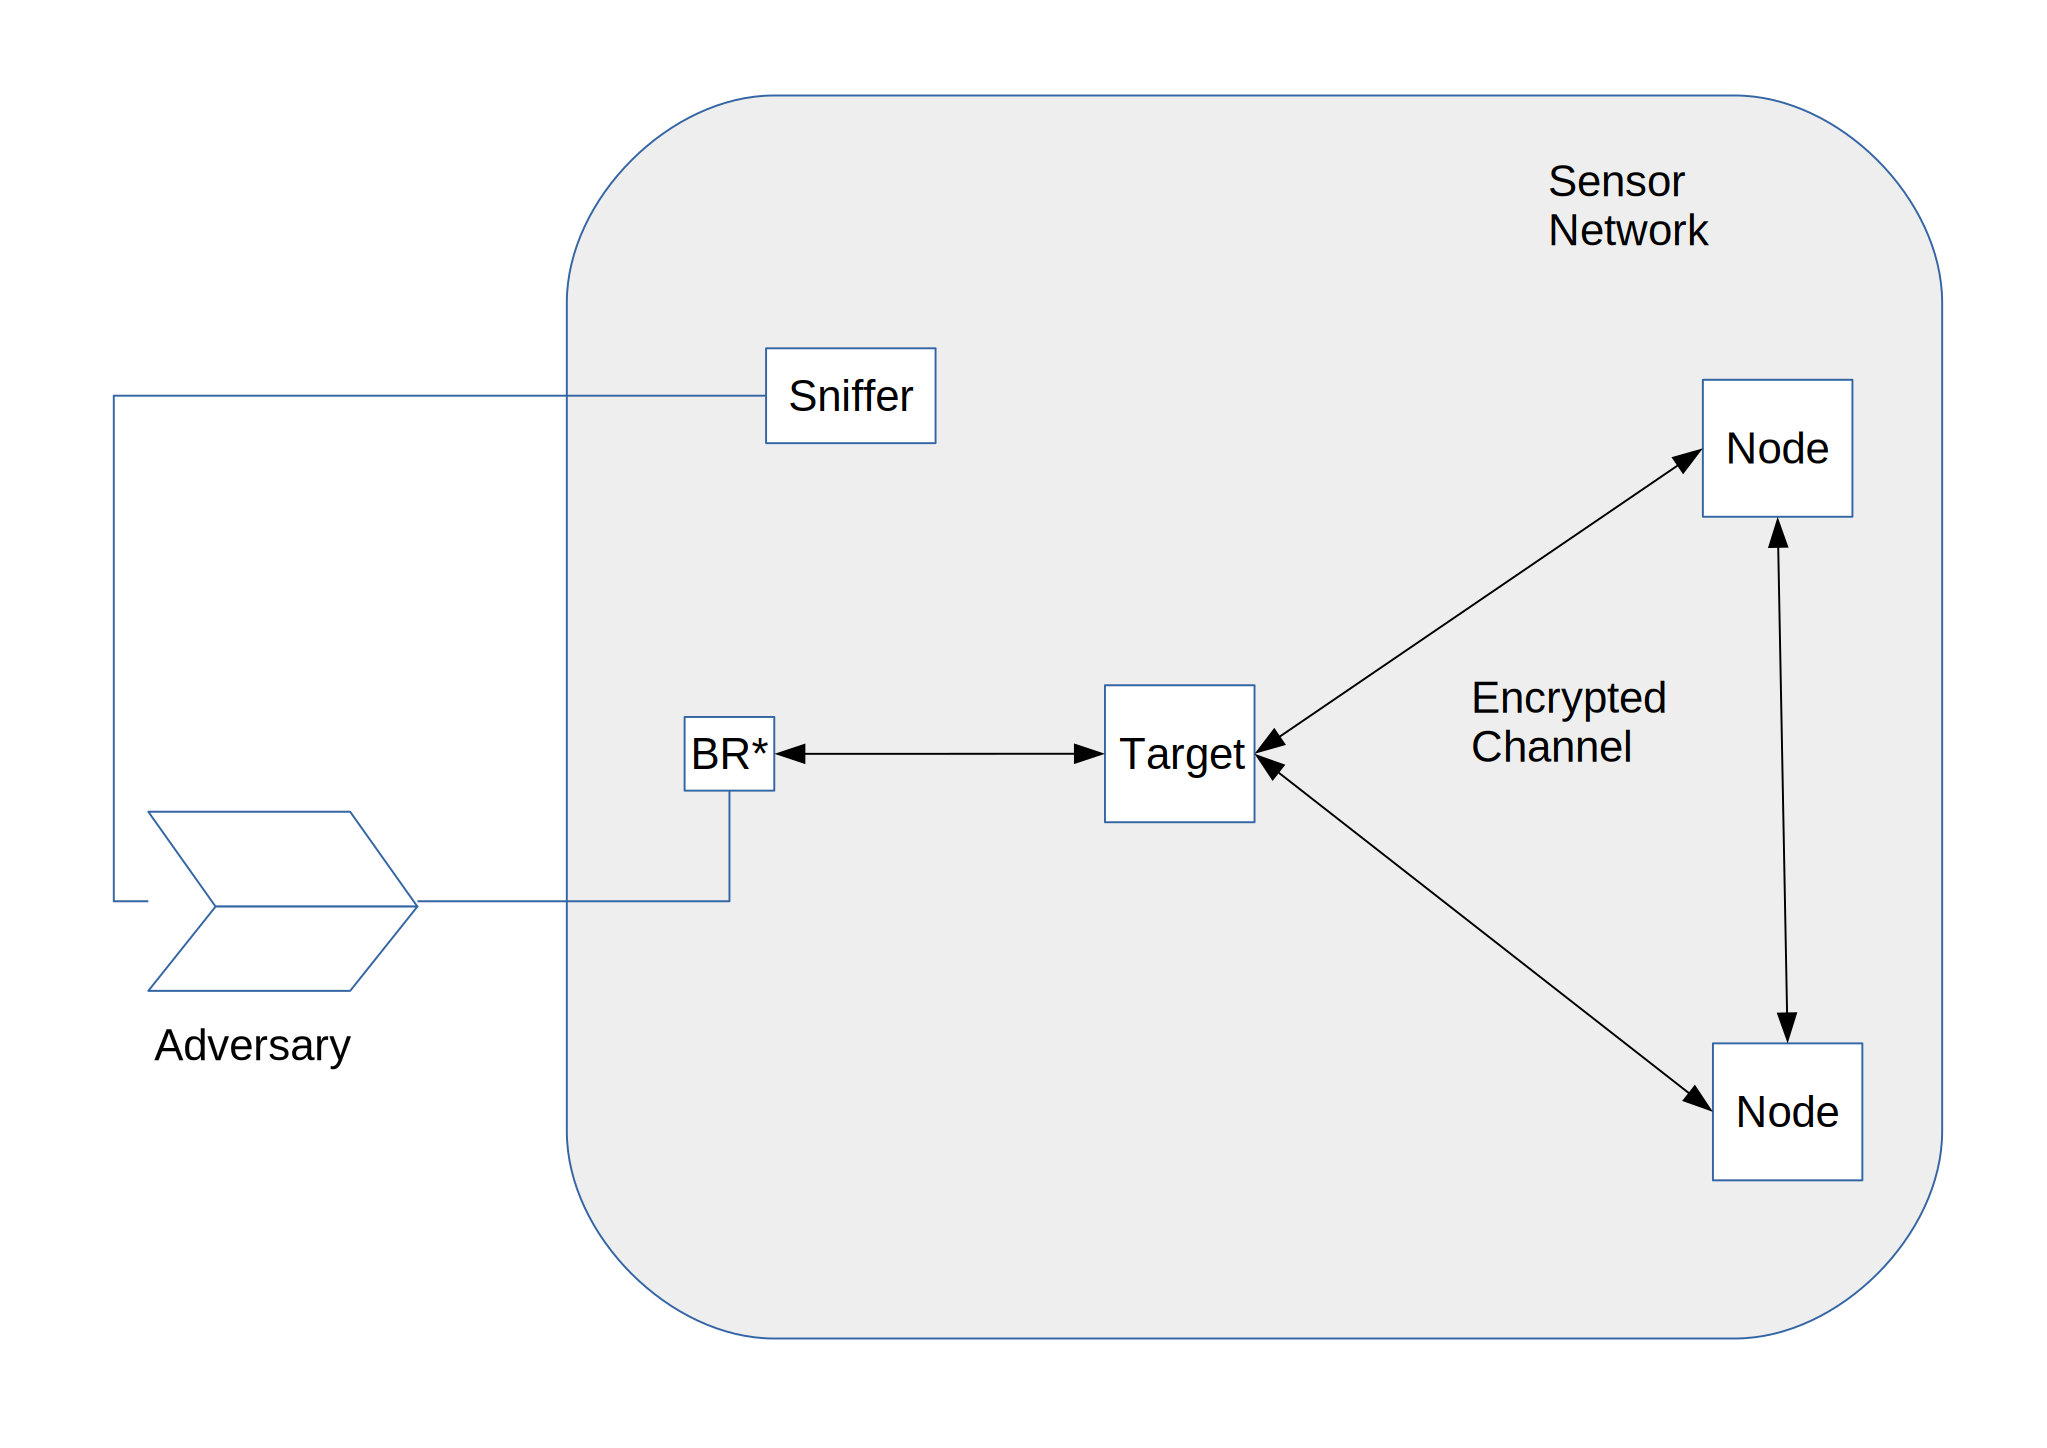
\includegraphics[width=0.9\textwidth,]{fig/setup.png}
	\caption{Experiment Setup} \label{Fig: Experiment Setup}
\end{figure*}

\begin{description}[style=nextline]
	\item[Sensor Network]
	The greyed area on the right inside the rectangle of \Cref{Fig: Experiment Setup} represents a WSN application.  The topology is dynamic and can change due to the application.  We make no further assumptions about the exact application at this point for generality.
	
	\item[Sensor Node]
	Each Sensor Node is a device with support of the protocol suite described in \Cref{Tbl: Summary of WSN Building Blocks}. All Sensor Nodes are connected to the same 6LoWPAN network. We do not impose the use of CoAP in our setup; instead, we assume applications may directly use the interface of UDP( or DTLS). More details are  are given in the later sections.
	
	\item[Border Router]
	Border Router is a special instance of Sensor Node. In addition to RF, Border Routers are additionally connected to other devices via different connections. In the experiments of this project, Border Routers are connected to a laptop through a USB connection. Border Router bridges two network. In the scenario of \Cref{Fig: Experiment Setup}, the Border Router is used to transmit IPv6 packets sent from the laptop. From a perspective of other Sensor Nodes in the WSN, a Border Router appears no different to the others. In many real world applications, the Border Router is connected to a management machine and serves as the DODAG root but this is not necessary in this experiment.
	
	\item[Sniffer]
	Sniffer is another special instance of Sensor Node. The Sniffer passively captures all frames it receives and does not transmit anything at all; thus it is transparent to other Sensor Nodes in the network. In our setup as of \Cref{Fig: Experiment Setup}, the Sniffer pipes any frames it captured to the Laptop. From a practical perspective, the hardware device of a Sniffer has a limited effective radius and thus would not be able to capture all frames in WSNs of wide deployment; however this can be easily overcame by deploying multiple synchronised Sniffers to cover a wide area. In our experiments, we assume every frame in the network is captured by the Sniffer.
	
	\item[Laptop]
	The Laptop in our experiment represents an adversary with unequally supreme resources comparing to the Sensor Nodes in terms of energy, memory and computational power. In our setup of \Cref{Fig: Experiment Setup}, the Laptop, which also represents the adversary, has access to all traffic captured by the Sniffer and is allowed to interact with other Sensor Nodes through the Border Router if authentication is not required to join the network.
\end{description}

\section{Operating System}

We use Contiki\cite{Contiki} to build our experiments.  Our source code are tested  with the release version of Contiki 3.0 which is available at:

\begin{center}
	\url{https://github.com/contiki-os/contiki/releases/tag/3.0}.
\end{center}

\subsection{Brief Introduction to Contiki:}

The official instruction for using Contiki is available at:
\begin{center}
	\url{http://www.contiki-os.org/start.html}
\end{center}

Contiki is an open source embedded system crafted for IoT devices. It has a good support on many recent hardware and it is optimised for code size. Comparing to Operating Systems for PCs, Contiki does not provide a User Interface, UI. Instead, the embedded system provides a framework for developers to use C language to write (mostly) hardware portable codes, as well as a set of APIs including clock library, simple process management and network interfaces,etc.

To use Contiki, there are basically three steps:

\begin{enumerate}
	\item Write the application code in C. There are plenty of code in the Contiki example folder that can be used as frameworks.
	\item Compile the source code according to the target device through \textit{make} command. Note that the root of Contiki source code must be correctly specified in the \textit{makefile}.
	\item Upload (also called ``burn'') the binary code to your device. 
\end{enumerate}

The application code is automatically executed whenever the device is powered on.

\section{Devices}

Three models of device are adopted in this project:

\begin{itemize}
	\item \textbf{TelosB}\cite{TelosB}, as known as Sky mote. This is a popular model for WSNs featuring low cost. As a trade off, TelosB has only very constrained performance in terms of bandwidth, available code size and processing power.
	
	\item \textbf{CC2538}\cite{CC2538}. This is a relatively powerful model with an ARM-Cortex M3 processor. To our knowledge, this is one of the becoming dominant device used in WSN applications.
	
	\item \textbf{Wismote}\cite{Wismote}. This model is used as a performance upgraded version of TelosB in this project. In this project, Wismote \textbf{IS ONLY USED IN SIMULATIONS}. 
\end{itemize}

All these nodes are 802.15.4\cite{802154} compatible and does not have any sensor attached by default. We omit further hardware details as it is beyond the scope of this project. 

\subsection{Cooja Simulator}

The Contiki source code includes the Cooja simulator under its tools folder. The official instruction of using the Cooja simulator is available at 

\begin{center}
	\url{http://www.contiki-os.org/start.html}
\end{center}

Cooja provides simulation for a whole WSN application. It generates simulation data for serial output, LED status and radio traffic. An example of Cooja execution is shown in \Cref{Fig: An Example of Cooja Execution}.

\begin{figure*}[h!]
	\center
	\includegraphics[width=0.8\textwidth]{fig/cooja_example.png}
	\caption{An Example of Cooja Execution}
	\label{Fig: An Example of Cooja Execution}
\end{figure*}

\Cref{Fig: An Example of Cooja Execution} shows a simulation simulating the exact same WSN topology as described in \Cref{Fig: Experiment Setup}, with \textcircled{1} being the Border Router. 

In this project, we are mostly interested into the radio traffic, captured by the ``Radio messages'' plug in which acts as the Sniffer in \Cref{Fig: Experiment Setup}. The corresponding pcap file is written by Cooja alongside the simulation under ``cooja/build/'' folder, which can later be opened by Wireshark\cite{Wireshark} for analysis, as shown in \Cref{Fig: A Wireshark Example}.

\begin{figure*}[h!]
	\center
	\includegraphics[width=0.8\textwidth]{fig/wireshark_example.png}
	\caption{A Wireshark Example}
	\label{Fig: A Wireshark Example}
\end{figure*}

As of the time of writing this report, Cooja in Contiki release 3.0 supports simulation for TelosB and Wismote. CC2538 is not yet supported by the current version.

\section{Security Protocols}
\subsection{LLSEC}

\subsection{DTLS}

\section{Applications}


%\begin{itemize}
%\item{\bf Adversary} is a malicious party that tries to illegally reveal information from the encrypted traffic.
%\item{\bf Border Router}, or BR, is a device that connects adversary to the sensor network. \textbf{BR is not allowed when LLSEC is enabled} as the adversary does not have the key and hence cannot connect into the network. We will discuss more about LLSEC in \Cref{Chp: LLSEC}.
%\item{\bf Sniffer} passively captures all traffic in the network. 
%\item{\bf Target} and {\bf Nodes} are sensors deployed in the sensor network. They communicates to each other through encrypted channels.
%\item{\bf Sensor Network} discussed in this paper is a 6LowPAN network based on Contiki OS.
%\end{itemize}

%Realistically speaking, this scenario could happen say an adversary sitting near a smart house with a laptop attached to a SoC\footnote{System on Chip} device, or your malicious neighbour walks into your smart house with her smart phone.
%
%\section{Adversary Power}
%The powers assumed in the experiments are considered to be practical in real life.
%
%When LLSEC is enabled, all traffic, including RPL\footnote{Routing Procol for Low-power and Lossy Networks} messages, are encrypted; therefore no external nodes can connect to the network as an external node cannot send any valid RPL messages to join the network. The adversary only passively sniffs all traffic.
%
%With LLSEC disabled, the adversary can therefore join the sensor network through a BR and hence is also capable to send messages to the target(s). However, she will not be able to inject any message into an encrypted channel such as a DTLS channel.
%
%\section{Types of Packets}
%We simply categorise the packets into two types:
%\begin{itemize}
%\item {\bf Network Management Packets}: These are the packets generated by the protocols to  maintain the functionality of network, such as MAC ACKs, RPL messages or ICMP messages.
%\item {\bf Data Packets}: These are those packets generated by applications running on sensor nodes., such as a CoAP packet.
%\end{itemize}
%
%This is only a subjective rough categorisation and may not be precise. For example an TCP data packet may set its ACK flag, or DTLS handshake packets could ambiguously fall into both categories. However, we ignore this ambiguity as it is not our focus.
\chapter{Potential Leakage Sources}

In this chapter, we discuss the potential leakage sources in the environment we have set up in \Cref{Chp: Experiment Setup}. 

\section{Subject} \label{Sec: Subjects}

Without loss of generality, in this report, we are interested in leakages with respect to the following subjects:

\begin{itemize}
	\item Content and size of encrypted data
	\item Cryptographic key materials
	\item Network topology
\end{itemize}

In this chapter we give a theoretical analysis of the exploitable side channel information in the WSN traffic. The inspection of protocol and implementation flaws are included in later chapters.

Notice that Traffic Analysis is highly application specific. In this report, our discussions are based the simple applications described in \Cref{Sec: Applications}. 

\section{Observables} \label{Sec: Observables}

As we have explained in \Cref{Chp: Experiment Setup}, we assumed the adversary has full access to all traffic being transmitted in the WSN. 

\begin{figure*}[h!]
	\center
	\includegraphics[width=0.9\textwidth]{fig/udpexample.png}
	\caption{An Example of Captured Traffic}
	\label{Fig: An Example of Captured Traffic}
\end{figure*}

\Cref{Fig: An Example of Captured Traffic} shows the packets captured in a Cooja experiment, analysed by Wireshark\cite{Wireshark}. In this research, we assume the value of ciphertext is independent to the plaintext and key. The following side channel information are available in the captured traffic shown in \Cref{Fig: An Example of Captured Traffic}:

\begin{description}[style=nextline]
	\item[Timing]
	Time of each packet sent is shown at the Time column on the upper half of \Cref{Fig: An Example of Captured Traffic}.
	\item[Packet Size]
	Packet size is shown in the Length column in the upper half of \Cref{Fig: An Example of Captured Traffic}.
	\item[Unencrypted headers]
	This is shown in the bottom half of \Cref{Fig: An Example of Captured Traffic}. The highlighted packet is a DTLS Data Record. We can see that the available headers are physical information (Frame), 802.15.4 MAC Header (IEEE 802.15.4 Data), compressed IPv6 Header (6LoWPAN and Internet Protocol Version 6), UDP Header (User Datagram Protocol) and DTLS Header (Datagram Transport Layer Security). Details of headers are shown under each tab.
\end{description}

Timing and packet size are always available in the captured traffic. The unencrypted headers depend on the security measure being used, which we explain in later sections.

Practically, the Receive Signal Strength Indicator, RSSI, should also be considered visible to the adversary. RSSI represents the RF signal strength. By measuring the RSSI of frames sent from a specific MAC source address,  it is possible for the adversary to reveal the geographical information of a specific Sensor Node. However we do not consider RSSI in this report as its physical character is beyond the scope of this report. Instead, we assume the adversary has prior knowledge of all geographic information of Sensor Nodes in the WSN.

\section{Packet Traces} \label{Sec: Packet Traces}

In this section, we explain some features of WSN traffic traces comparing to Internet applications.

Design of WSN applications tends to be simple and stateless due to the nature of constrained resources and unreliable transmission. As a result, data exchange is minimised for efficiency and robustness. From this aspect, we argue that our simple applications in \Cref{Sec: Applications} have captured these most significant characteristics of WSN applications.

In this report, we define a generic model for the data exchanging process in WSN applications.

\begin{definition} \label{Def: Session}
A Session is defined as a series of events where a Sensor Node reports application data to a Manager. A Session includes an optional Request sent from Manager to Sensor Node, and a Response containing the requested data sent from Sensor Node to Manager.
\end{definition}

\Cref{Fig: Overview of Session} shows an overview of a Session. Practically, the Manager can be a specific Sensor Node in the WSN, or a desktop connected to the WSN through a border router.

\begin{figure*}[h!]
	\center
	\includegraphics[width=0.8\textwidth]{fig/Session.png}
	\caption{Overview of Session}
	\label{Fig: Overview Session}
\end{figure*}

\begin{definition} \label{Def: Trace}
A trace is all captured packets within one Session.
\end{definition}

Although not necessary under \Cref{Def: Session}, in most of our applications, there are typically one or two packets in a trace. The first one corresponds to Request and the second corresponds to Response. In some applications such as broadcast keyllsec or a CoAP application using OBSERVE option, there might be only one Response packet in a trace without a Request. In real world applications there might even be a Request without a Response, e.g. a command to control a light bulb. However, in this report, we define there is at least one packet corresponds to Response. We further assume the adversary is aware of the application running on the Sensor Nodes. Consequently, the adversary in our setting is able to distinguish a Request and a Response, but has no knowledge of the application data being transmitted within them.

We also assume the adversary is capable to distinguish Sessions. Practically, the time interval of packets within the same Session are usually significantly less then the interval between Sessions. \Cref{Fig: Example Traces of keyllsec} shows an example of traces in a unicast keyllsec application instance. Marked are packets from two continuous Sessions, where No.977 and No.990 are from the first Session and No.998 and No.1011 are from the second. We can see that the time interval within a Session is about 150ms which is significantly less than the 15s interval between Sessions.

\begin{figure*}[h!]
	\center
	\includegraphics[width=0.5\textwidth]{fig/unicast_keyllsec.png}
	\\
	\includegraphics[width=0.9\textwidth]{fig/trace_keyllsec.png}
	\caption{
		Example Traces of keyllsec, \textcircled{1} is the sender and \textcircled{2} the receiver.
	}
	\label{Fig: Example Traces of keyllsec}
\end{figure*}

%The following paragraph is removed as the focus is shifted from application data to RPL messages.
%In this project, we consider only information leakage within one Session. Arguably, there could potential leakage when jointly analyse traces from different Sessions, e.g. the frequency of Requests can ``leak'' itself. However, we omit such leakage for generality as exploiting them requires further assumptions to the higher level application. Each Session in this report is also considered to be independent based on that fact that each execution of our code is independent to its last execution.

%Further more, in our applications the content of Request is a constant 3 bytes ASCII string ``GET''. We assume this known by the adversary. We make this assumption to focus on the leakage of the Application Data in Responses. 

\section{Theoretical Analysis} \label{Sec: Theoretical Analysis}

In this section we provide a theoretical analysis over all observables we explained in \Cref{Sec: Observables}. It is done in two approaches:

\begin{enumerate}
	\item Cross reference the observables with the exploited side channel information we introduced in \Cref{Sec: Traffic Analysis Attacks}
	\item Semantically analyse the observables. 
\end{enumerate}

%We discuss only the leakage over the attributes we specified in \Cref{Sec: A Review of Review}.

For some observables, we claim:

\begin{theorem} \label{Te: IR}
Under the leakage definitions of Mutual Information and g-leakage in \Cref{Subsec: Information Theory}, if an observable $Y$ is independent to a secret $X$, then there is $0$ leakage of $X$ over $Y$.
\end{theorem}

\Cref{Te: IR} intuitively holds. A formal proof is given in \Cref{Prf: IR}.

\begin{corollary} \label{Cor: Constant Leakage}
	An observable $Y$ with a constant value has no leakage under the leakage definitions of  Mutual Information and g-leakage in \Cref{Subsec: Information Theory}.
\end{corollary}

\begin{proof}
	This directly followed by the fact that a constant $y \in Y$ with $P(y) = 1$ is independent to the secret $X$.
\end{proof}

\subsection{Cross Reference of Observables with Known Attacks} \label{Subsec: Cross Reference}

Among all packet features we summarised in \Cref{Tbl: Classifiers in Traffic Analysis Literatures}, we only found four applicable in our WSN setting:
\begin{itemize}
	\item Packet size
	\item Total bytes
	\item Total Time (only for two packets Session)
	\item Total Per-direction Bandwidth
\end{itemize}

All other features have reduced to a constant or not applicable in our settings. The detailed analysis is described in \Cref{Detail Cross Reference}.

\subsection{Semantic Analysis}

In this section, we analysis the observables in \Cref{Sec: Observables} based on their semantics. The contents of headers can be referred to \Cref{Chp: Building Blocks}.

\subsubsection{Packet Size}

%Linear relationship of length
We noticed that both noncoresec and DTLS use AES-128 with CCM mode to encrypt their payload. The data is therefore not padded due to the nature of a stream cipher. This effectively indicates that the length of a plaintext $l_P$ is expected to be linear to the length of its corresponding ciphertext $l_C$:

\begin{equation} \label{Eq: Linear Length}
	l_{C} = l_{P} + b
\end{equation}

where $b$ is a predictable constant induced by security measures such as MIC and additional headers.

Practically when the security measure increases the packet size to a value exceeding MTU, the packet will be immediately dropped. We assume plaintext is always in a reasonable length that does not result into a ciphertext exceeding MTU; otherwise the packets cannot be sent and the WSN loses its functionality.

From a leakage perspective, it is obvious that all bits of $l_P$ is leaked by $l_C$. A formal quantification of this leakage is given in \Cref{Linear Leakage}.

\subsubsection{Timing}

Timing information is another important side channel information in WSN traffic. Comparing to Internet applications, we consider timing information as a even more crucial leakage source in WSN for two reasons:

\begin{enumerate}
	\item The timing can be measured more accurately in WSN. Packet traces on Internet are usually measured at one side of the communication where the noise induced by RTT must be considered, whilst timing of every packet forwarding is known in our setup.
	\item The low performance of the WSN devices potentially increases the resolution of timing information. Any differences of execution time will be more distinguishable on these devices.
\end{enumerate}

However, timing information would be hard to exploit without precise knowledge of the code running on the target Sensor Node. Several protocol may also affect the measurement, .e.g. ContikiMAC turns off the radio for most of the time and therefore preprocessing is required to measure the exact timing of each packet in the traces.

\subsubsection{Unencrypted Headers with noncoresec}

When noncoresec is enabled, the 802.15.4 MAC Header is the only visible part in all Data Frames. We have not identify any obvious leakage source in the MAC Header that links to our applications. 

%Address
However, in the experiments we realised that the Address Information combined with some other packet features can be used distinguish the RPL messages from the application packets. We discuss more details in later chapters.

Details of the semantic analysis of 802.15.4 MAC Header is given in \Cref{Detail noncoresec Header}. 

\subsubsection{Unencrypted Headers with DTLS}

DTLS is built over UDP; therefore visible headers are 802.15.4 MAC header, compressed IPv6 Header, UDP header and DTLS header. We neither found any obvious value that links to our application data.

However, there are two points need to be awared within DTLS:
\begin{enumerate}
	\item Currently DTLS does not support any form of multicast; therefore when DTLS is used, the destination address can only be a unicast address. 

	\item DTLS protects only application data, the ICMP messages, including RPL messages, are transmitted in plaintext.
\end{enumerate}

Even though DTLS can only be used on unicast communications in our applications, proposals such as \cite{DtlsMulticast1} \cite{DtlsMulticast2} has been made to adapt DTLS to multicast; therefore it is reasonable to expect that the family\footnote{Unicast and multicast. Broadcast is treated as an instance of multicast in IPv6.} of destination address can be a hint to the contents of data encrypted by DTLS in the future. However, we do not discuss this topic further as multicast on DTLS is not implemented yet.

Also to be noticed is that the size of compressed IPv6 Header is variable. Since most of the options are not available in our platform, the variance is most likely to be caused by the use of different modes of addresses. However, all our experiments are set up with the same mode addresses and therefore the compressed IPv6 Header effectively resulted into a constant size.

Details of semantic analysis of the visible headers within DTLS is given in \Cref{Detail DTLS Header}. 

\subsection{Conclusion}

In conclusion, the packet size and timing information are still likely to be the most exploitable side channel information in WSN, just as those attacks on Internet. However, the address information is a potential leakage source in WSN applications.

\section{Leakage of Network Topology} \label{Sec: Leakage of Network Topology}

As explained in \Cref{Sec: Observables}, the geographical information of Sensor Nodes can be detected from the RSSI. Based on this information, topology of the 6LoWPAN network can be deduced in the following ways:

\begin{enumerate}
	%With noncoresec
	\item Within noncoresec, the RPL messages are encrypted. However, the source and destination address information is still visible to the adversary; therefore the connectivity between Sensor Nodes can be estimated based on these information.
	%With DTLS
	\item Within DTLS, the RPL messages are not encrypted. The adversary can reconstruct the network topology from the captured RPL messages.
\end{enumerate}

\section{Summary}

In this chapter, we started by specifying the subjects of information leakage, namely the content and size of application data, cryptographic key materials and network topology in \Cref{Sec: Subjects}. Then we demonstrated an example of captured data and pointed out the available information to an adversary in \Cref{Sec: Observables}. From there, we provided a definition of Sessions in WSN applications and the discussed the form of packet traces in our applications in \Cref{Sec: Packet Traces}.

In \Cref{Sec: Theoretical Analysis}, we gave a theoretical analysis of the observables in WSN traffic. Packet size and timing information turned out to be the likely most exploitable feature even in WSN, while unencrypted address information can also be a hint to the contents in the encrypted data.

With respect to network topology, the unencrypted 802.15.4 MAC Header within noncoresec can be used to estimate the connectivity between Sensor Nodes. DTLS does not protect the RPL messages thus an adversary can reconstruct the network topology from the RPL messages transmitted in plaintext.
%\chapter{Link Layer Security: noncoresec} \label{Chp: LLSEC}

In this chapter, we provide an analysis for the Link Layer security measure noncoresec, which we have explained in \Cref{Subsec: 802.15.4 Security Implementation in Contiki}.

\section{Protocol and Implementation}
%Reset Problem
In this section, we analysis the noncoresec implementation with respect to the problems described by \cite{802154sec}. 

\subsection{Nonce Reuse}

As we have explained in \Cref{Subsec: 802154 Nonce}, the only variable field in the nonce is Frame Counter. Since noncoresec only supports network shared key, there are two potential problems according to \cite{802154sec}, namely nonce reuse and anti replay. Further inspecting the source code, we realised that the counter is declared as a static value and is initialised to $0$ on each reboot.

Our experiments confirmed the vulnerability. We simulated two executions of  broadcast\_example of keyllsec in \Cref{Sec: Applications}, broadcasting the same message. Our data\cite{NonceReuseData} showed that frames with the same Frame Counter results into the same ciphertext. In reality, this vulnerability implies that an adversary capable to reset the device can eventually learn the difference in plaintext by calculating the difference of ciphertext with the same Frame Counter, causing severe breach of data confidentiality.

One solution might be to store part of the Frame Counter on the flash and increases that value on each time reboot. Assume the device averagely sends one frame every minute stores the highest byte of Frame Counter, it is resilient in $2^8$ reboots and the lower bytes still has the space of $2^{24}$ frames, which holds up to nearly 32 years. Another solution could be to set the higher bytes of Frame Counter to a random value on each reboot. For example, by setting the highest byte to a uniformly distributed random value in $[0,255]$, the adversary is expected to successfully reset the Frame Counter to a specific value with probability of $2^{-8}$ on each reboot.

\subsection{Anti Replay}

\cite{802154sec} has pointed out that anti replay in 802.15.4 Security is incompatible with network key as the same ACL entry is shared among multiple nodes, causing confusion of Replay Counter in ACL. However, with an inspection of the source code of Contiki, we realised that the noncoresec does not suffer the same problem as the ACL is not implemented; instead, a similar data structure is added to the routing table in kernel  associated to each source address.

\section{Common Analysis}

%Packet Length

%Timing for encryption

%RPL Messages

%Sequence Numbers

\section{Application Analysis}




%
%Link Layer Security, or LLSEC, is a security measure that implements cryptography at Data Link Layer\footnote{https://en.wikipedia.org/wiki/OSI\_model} which is only above Physical Layer.
%
%Introducing cryptography at a lower level has several benefits. Firstly, more data being encrypted reduces the observable packet features to an adversary, such as SRC\footnote{Source Address} and DST\footnote{Destination Address} field in the IP header which are very likely to be exploited by an adversary. Secondly, authentication at lower level also prevents an active adversary from joining the network which therefore weakens her power. 
%
%On the other hand, imposing cryptography at a lower level also brings more challenge to the design of sensor network architecture. The first problem is its overhead. For example, even for a node that only forwards a packet to its next hop, it must decrypt the whole packet to extract its routing information, and then re-encrypt it before transmission. This is particularly problematic in a mesh wireless sensor network as it could potentially downgrades the performance and causing energy consumption problems. More over, key management is also challenging due to the constrained computational power and power optimised lossy nature of wireless sensor network.
%
%It is noticeable that some packet features are not hidden even with LLSEC enabled, such as packet length, timing information and part of the MAC header in a 802.15.4 packet.
%
%\section{802.15.4 Security: {\it noncoresec}} \label{sec: noncoresec}
%{\it noncoresec}\cite{LLSEC} is the current implementation of LLSEC in Contiki. It implements AES\_CCM\_16 ciphersuite in 802.15.4 standard. This section briefly describes how it works.
%
%\begin{itemize}
%\item {\bf Key Management}: All nodes share a network wide AES key for both encryption and authentication. The key is hardcoded during the setup stage.
%
%\item{\bf AEAD\footnote{Authenticated Encryption with Associated Data}}: {\it noncoresec} implements AES\_CCM\_16 \footnote{CCM mode of AES-128 with 16 bytes MAC} as described in 802.15.4\cite{802154} which turns AES into a stream cipher. The same key is used for both encryption and authentication.
%
%\item{\bf Initial Vector (IV, or nonce)}: The IV for each packet is constructed from certain fields of unencrypted MAC header and therefore is public.
%\end{itemize}
%
%An adversary without the knowledge cannot join the sensor network protected by \textit{noncoresec} as she cannot sent out a valid RPL message.
%
%\section{Weak IV}
%
%\begin{figure}
%\centering
%\begin{tabular}{| l | l | l | l | l |}
%\hline
%Flags(1) & Addresses(8) & Frame Counter(4) & Security Level(1) & Block Counter(2)       \\ \hline
%\end{tabular}
%\caption{IV of 802.15.4 Frame with Security} \label{Tbl: 802154 Frame}
%\end{figure}
%
%One problem within the {\it noncoresec} implementation is the low variance of IV. The IV is a $16$ byte bit-string constitutes of the following fields(\Cref{Tbl: 802154 Frame}):
%\begin{itemize}
%\item {\bf Flags (1 byte)}: This field contains part of the MAC header. It is identical to most (basically all) of the data packets.
%
%\item{\bf Source Address (8 bytes)}: This is mapped from the source address field of the packet.
%
%\item{\bf Frame Counter (4 bytes)}: This field increases by 1 from 0 for each packet sent to prevent replay attack.
%
%\item{\bf Security Level (1 byte)}: This field indicates which ciphersuite to be used for this packet. In the case of AES\_CCM\_16, this is constantly 0x7.
%
%\item{\bf Block Counter (2 bytes)}: This field begins from 0x0 and increases by 0x1 for each block in CCM mode. The block length for AES-128 is 16 bytes. The 2 bytes counter is usually sufficient as it supports up to $2^{32}$ bytes of data whereas the minimum MTU\footnote{Maximum Transmit Unit, simply speaking this is the maximum length of a packet.} required by 6lowPAN standard\cite{rfc4944} is $127$ bytes.
%\end{itemize}
%
%In the current {\it noncresec} implementation, \textbf{Flags} and \textbf{Security Level} are constant. \textbf{Block Counter} always begins from 0x0 and the \textbf{Source Address} is also constant for a specific device. Such design leaves the 4 bytes \textbf{Frame Counter} the only field that is variable. This indicates that only $2^{32}$ messages are allowed without a collision of IV which is cryptographically considered to be inappropriate.
%
%\subsection{Reset Problem}
%The low variance of IV leads to a plaintext leakage problem which only requires the adversary to reboot the target node. 
%
%The idea is that rebooting the device resets the \textbf{Frame Counter} to 0x0; hence once a pair of packets with same \textbf{Frame Counter} is found, the difference of their plaintext can be computed by their ciphertext:
%\begin{equation*}
%\Delta p = c_1 \oplus c_2
%\end{equation*}
%where $\Delta p$ is the difference of plaintexts. $c_1$ and $c_2$ are their ciphertext respectively.
%
%\begin{example}
%\begin{figure*}
%\centering
%{
%	\includegraphics[width=0.9\textwidth,]{fig/resetproblem.png} 
%}
%\caption{Captured packets with {\it noncoresec} enabled} \label{Fig: reset problem}
%\end{figure*}
%
%\Cref{Fig: reset problem} demonstrates some packet captured\footnote{The duplicated packets are caused by the retransmission of ContikiMAC\cite{ContikiMAC}.} with {\it noncoresec} enabled. These packets are captured with a sensor broadcasting a 4 byte integer with left side of \Cref{Fig: reset problem} being $[00000000]_{16}$ and right $[12345678]_{16}$. Marked are the corresponding ciphertexts which are $[00127401]_{16}$ and $[12262279]_{16}$ respectively.
%
%As we can see, the difference of ciphertext is exactly the difference of plaintext:
%\begin{equation}
%\Delta p = [00127401]_{16} \oplus [12262269]_{16} = [12345678]_{16}
%\end{equation}
%\end{example}
%
%\section{Distinctive Packet Length for RPL Packets}
%Some RPL packets are shorter than the minimum length of data packets which can be used to distinguish the packets. Further more, some RPL packets set MAC header flags differently from data packets.
%
%\section{Performance Issue}
%The header overhead with LLSEC enabled is 20 bytes which is relatively a large overhead comparing to the 127 bytes MTU requirement of 6LowPAN standard\cite{rfc4944}.
%\chapter{DTLS}



\section{Conflicting MTU between DTLS and 6lowPAN}
The abandoned CoDTLS.
\section{Overloading DTLS with LLSEC}
%\chapter{Application Detection}
Similar to website fingerprinting, we try to identify the application running on target note by its traffic. This chapter discusses some general idea without a specific application.

\section{Network Protocol Headers}
Since most information in MAC\footnote{Media Access Control, not to be confused with the cryptographic term Message Authenticate Code.}, IP and UDP headers are related to routing and network maintenance and thus independent except the length fields and CRC\footnote{Cyclic Redundancy Check, a code to detect or correct transmission error}. 

\section{Packet Length}
Packet length is usually the most interested target in traffic analysis. However, packet lengths are also highly application dependant; thus we are not pursuing this topic further without a specific application.

\section{Timing Packet Response}
Unlike web applications where the client and server are usually physically distant, sensor networks can sometimes located in a concentrated area, such as a house which its radius can be less than 10 meters. 

These features theoretically enables one to capture all traffics in such a sensor network. As opposed to the case of Internet where packets are usually timed on the client’s side and thus network latency (RTT\footnote{Round-Trip Time}) must be concerned, being able to capture all traffic in the network provides  much more accurate timing information and hence may be exploited to develop more efficient attacks.

\begin{definition}
In a Request-Response application model, \textbf{RI}, {\bf Response Interval}, is defined as the interval between a request packet being received and its response being sent.
\end{definition}

\begin{example}
\begin{figure}
\centering
{
	\includegraphics[width=\textwidth,]{fig/responsetime.png}
}
\caption{Capture of a ping packet}
\label{fig: ping packet}
\end{figure}

\begin{table}[!]
\centering
\begin{tabular}{|l|l|l|l|l|}
\hline
Time (ms) & From (ID) & To (ID) & Length (bytes) & Type          \\ \hline
1961218   & 1         & 2       & 108            & ICMP ECHO \\ \hline
1961222   & 2         & 1       & 5              & 802.15.4 ACK  \\ \hline
1961230   & 2         & 1       & 107            & ICMP ECHO \\ \hline
\end{tabular}
\caption{Packet Features of an ICMP ECHO request and response}
\label{Tbl: ping}
\end{table}

Three packets are marked out in \Cref{fig: ping packet} which forms an instance of ICMP ECHO\cite{rfc1122} (also known as PING) session. The extracted packet features are displayed in \Cref{Tbl: ping}.

\begin{description}
\item[Explanation of the Packets:]\hfill \\
The first packet is an ICMP ECHO request and the third packet being its response. The second packet is a 802.15.4 ACK\footnote{This is an acknowledgement from the receiver that notifies the sender that the packet has been received.} and is thus transparent to the upper ICMP protocol.
\end{description}

From this example we can see that the RI for this PING session is:
\begin{equation*}
1961230 - 1961218 = 12 \text{(ms)}
\end{equation*}

\end{example}

Timing information can be exploited by several attacks, such as \cite{Peekaboo} and \cite{rsatiming}.

We have experimentally measured a RNG\footnote{Random Number Generator} call on Wismote platform in the Cooja simulator is roughly 0.3 ms.

\section{PINGLOAD: PING side-channel for Payload }
Support of ICMP ECHO is required by \cite{rfc1122} and is also enabled in Contiki OS by default. However, our experimental results shows that the response time of these ping packets could potentially be exploited to reveal the application running on target sensor node.

We call such technique {\bf  Application Fingerprinting}.

\subsection{Hypothesis}
A phenomenon we realised is that when a ping packet arrived while the target node is executing some payload, say reading a sensor or processing data, the PING RI begins to vary comparing to a stable value  when no there is no payload. 

\begin{example}
\begin{figure}
\centering
{
  \includegraphics[width=1\textwidth]{fig/pingri.png}
}
\caption{An example of PING RIs with different payload}
\label{Fig: PINGLOAD RIs}
\end{figure}
\Cref{Fig: PINGLOAD RIs} shows RIs of PING collected in two experiments. The upper half are collected with the target is constantly sleep whilst the lower half occasionally receives a request which triggers the target to call RNG. We can see that the PING RI varies alongside the target is given some payload from this figure.
\end{example}

The data shown in \Cref{Fig: PINGLOAD RIs} suggests that the “plain”, that is without any interference, PING RI is 12 to 13 ms. Further more, those variations of  PING RI is very likely caused by the payload of the target.

This experiment inspired that the distributions of PING RIs might vary according to the payload of target and could possibly considered as an fingerprint of the target’s application. In other word, an adversary could possibly tell whether the target is running a specific application by looking at its PING RIs distribution.

The attack is strait forward:
\begin{description}
\item[Profile sleep RIs]: \hfill\\
The PING RIs for a sleeping node of the same platform can be profiled by pinging a sleeping node. We denote the sleeping profile as $RI_{sleep}$. 

\item[Fingerprint application]: \hfill\\
The adversary collects PING RIs on a profiling node with known application. The profiling node needs to be of the same platform and executing the same code of the target’s. The application fingerprint denotes as: $F_p=\{p_1, p_2, ... , p_n\}$. 

\item[Collect fingerprint of target]: \hfill\\
The adversary then collects the PING RI for the target node by pinging it. We denote the collected data as: $F_t=\{t_1, t_2, ..., t_m\}$.

\item[Extract Featured RIs]: We can remove them from the data sets and keep the PING RIs those has been interfered by the application. We denote the extracted RIs as \textbf{Featured RIs}:
\begin{eqnarray*}
F’_p = \{x | x \in F_p,  x \notin RI_{sleep}\}\\
F’_p = \{x | x \in F_t,  x \notin RI_{sleep}\}
\end{eqnarray*}

Practically speaking, the PING protocol are designed to be responded immediately for diagnosis purpose; hence $RI_{sleep}$ usually has an extremely low variance and its mean is also much less than $F_p$ and $F_t$.

Using the Featured RIs not only provides a better vision of the fingerprint but also removes the error caused by different frequency of the target code being executed, as all the Featured RIs are actually collected when the node is at a non-sleeping state. 

\item[Estimate Distribution (Optional)]: \hfill\\
We then estimate the distributions of $F’_p$ and $F’_t$, denote as $D_p$ and $D_t$. A naive method is to simply use their histograms. An example of such histograms are shown as \Cref{Fig: featuredri_rng}.

\begin{figure}
\center
{
	\includegraphics[width=0.49 \textwidth]{fig/featuredri_rng1.png}
	\includegraphics[width=0.49 \textwidth]{fig/featuredri_rng2.png}
}
\caption{Two examples of RNG’s Featured RIs histogram}
\label{Fig: featuredri_rng}
\end{figure}

\item[Distinguish Distributions]: \hfill\\
Finally we test whether $D_t$ and $D_p$ are the same distribution. An naive way is to compute the correlation of counts of the histograms. We conclude the target node is running the profiled application if $D_t$ and $D_p$ are the same distribution.
\end{description}

Practically speaking, the key point of Application Fingerprinting is to test whether the target’s Featured RIs, i.e. $F’_t$, is sampled from same distribution of the profiled one, i.e. $F’_p$; therefore estimating their distribution might not be necessary for some statistical methods such as t-tests. However as we can see in \Cref{Fig: featuredri_rng}, PING RIs’ distribution are very unlikely to be normalised. Therefore a future work is to find a better distinguishing method than the current naive one.

\subsection{Experiment Result}
We tried our Application Fingerprinting method above on a Cooja simulated Wismote platform with different code. \textbf{In conclusion, the fingerprint appears to be effective for certain circumstances but will tends to result into false positives as the profiled application and target application gets similar to each other.}

To be more specifically, the target node execute some specific code upon receiving an application layer protocol request, similar to CoAP. Further more, all traffic are protected by DTLS with TLS\_PSK\_WITH\_AES\_128\_CCM\_8 ciphersuite. Both intervals of PINGs and the application request are set to some asynchronised value to avoid overflooding the target and to create a ‘more realistic’ simulation.

Everything other than the examined code are the same for all experiments. Two samples are collected independently for each code to simulate a fingerprinting scenario. The histograms are clustered by 5ms.

We examined two classes of codes:
\begin{description}
\item[RNG Calls]: \hfill\\
The target node repeatedly calls RNG for $i$ times. We examined their Featured PING RI for different values of $i$. The reason for picking RNG is that on some platforms where a hardware RNG is provided, the call to it is expected to be similar to a call to a sensor reading which is actually an interrupt. Results are shown in \Cref{Tbl: pingload RNG}.

\item[Arithmetic Operations]: \hfill\\
The target node repeatedly does arithmetic operations, namely addition, multiplication and modular, on two random generated word size integers for 10000 times. This class is particularly interested from a cryptographic point of view as the number of arithmetic operations could potentially developed to key recovering attacks. Results are shown in \Cref{Tbl: pingload arth}.
\end{description}



\begin{table}
\centering
\begin{tabular}{|c|cccc}
\hline
\textit{\textbf{Correlations}} & \multicolumn{1}{c|}{i=50} & \multicolumn{1}{c|}{i=100} & \multicolumn{1}{c|}{i=2500} & \multicolumn{1}{c|}{i=5000} \\ \hline
i=50                           & \textbf{0.988}            & 0.891                      & -0.014                      & -0.033                      \\ \cline{1-1}
i=100                          & 0.891                     & \textbf{0.973}             & -0.025                      & -0.042                      \\ \cline{1-1}
i=2500                         & -0.014                    & -0.025                     & \textbf{0.993}              & -0.035                      \\ \cline{1-1}
i=5000                         & -0.033                    & -0.042                     & -0.035                      & \textbf{0.985}              \\ \cline{1-1}
\end{tabular}
\caption{Correlations for RNG}
\label{Tbl: pingload RNG}
\end{table}

\begin{table}
\centering
\begin{tabular}{|c|ccc}
\hline
\textit{\textbf{Correlations}} & \multicolumn{1}{c|}{+} & \multicolumn{1}{c|}{*} & \multicolumn{1}{c|}{\%} \\ \hline
+                              & \textbf{0.990}         & \textbf{0.990}         & \textbf{0.988}          \\ \cline{1-1}
*                              & \textbf{0.990}         & \textbf{0.989}         & \textbf{0.985}          \\ \cline{1-1}
\%                             & \textbf{0.988}         & \textbf{0.985}         & \textbf{0.984}          \\ \cline{1-1}
\end{tabular}
\caption{Correlations for word arithmetic operations}
\label{Tbl: pingload arth}
\end{table}

\begin{table}[]
\centering
\begin{tabular}{|c|c|}
\hline
\textbf{\textit {Correlations}} & +     \\ \hline
i=50         & 0.877 \\ \hline
\end{tabular}
\caption{Correlation for $i=50$ and addition}
\label{Tbl: pingload rng arth}
\end{table}

We also computed the correlation for $i=50$ and addition, as shown in \Cref{Tbl: pingload rng arth}.

The results suggests the following conjectures:
\begin{enumerate}
\item The results for RNG suggests that the fingerprinting is effective for this class of code, as the same code results into nearly perfect correlations ($\geq 0.95$).

\item Even relatively slight changes can be detected, as we can see the correlation dropped to $0.891$ alongside 50 iterations of RNG calls (50 RNG calls take about 1.4ms).

\item The results for arithmetic operations indicates that their  fingerprint are unlikely to be distinguishable. There are two potential causes we have considered:
\begin{enumerate}
\item The differences between these operations are too small to be detected.

\item Experiment methodology error. Since the target node we used during the experiments call RNG twice upon each request to generate two operands whilst the word arithmetic operations have much lighter weigh comparing to RNG at magnitude level; thus the fingerprint is dominated by RNG rather than word arithmetic operations. As a result, we can see that a relatively high correlation can be observed between word addition and 50 RNG calls as shown in \Cref{Tbl: pingload rng arth}.
\end{enumerate}
\end{enumerate}

\subsection{General Hypothetical Model}
THE BLACK BOX MODEL
%\begin{table}[!ht]
\center
\begin{tabular}{|c|c|c|}
\hline
\textbf{Application} & \textbf{Trace Index} & \textbf{Note} \\ \hline
broadcast & 1 &  \\ \hline
broadcast & 2 &  \\ \hline
powertrace & 3 &  \\ \hline
powertrace & 4 &  \\ \hline
Sensorpayload & 5 & Temperature + Light \\ \hline
Sensorpayload & 6 & Temperature + Light \\ \hline
Sensorpayload & 7 & Temperature only \\ \hline
Sensorpayload & 8 & Temperature only \\ \hline
Sensorpayload & 9 & Light only \\ \hline
Sensorpayload & 10 & Light only \\ \hline
Sensorpayload & 11 & No reading \\ \hline
Sensorpayload & 12 & No reading \\ \hline
Sensorpayload & 13 & VDD only \\ \hline
Sensorpayload & 14 & VDD only \\ \hline
Sensorpayload & 15 & Temperature, Light and VDD \\ \hline
Sensorpayload & 16 & Temperature, Light and VDD \\ \hline
Sensorpayload & 17 & Light + VDD \\ \hline
Sensorpayload & 18 & Light + VDD \\ \hline
Sensorpayload & 19 & Temperature + VDD \\ \hline
Sensorpayload & 20 & Temperature + VDD \\ \hline
\end{tabular}
\caption{PingLoad Experiment Applications}
\label{PingLoadApps}
\end{table}

%\section{Conclusion}
In this paper we presented a study on the RNG design of CC2538. First, we revised the problem that using a 16 bit LFSR as PRNG is a bad idea and demonstrated how this design flaw can be exploited to break DTLS running on these devices. Secondly we presented a study to its seeding method and showed how such it could be remotely tampered by an adversary sending jamming signal to the device.

In fact the same RNG design has also been adopted many other products in the CC series including CC2420\cite{CC2420Manual}, CC2430\cite{CC2430Manual}, CC2520\cite{CC2520Manual} and CC253X, CC2540/41 series\cite{CC2530Manual}. We imagine all these products suffer the same problems. Fortunately the latest CC26XX/CC13XX\cite{CC26XXManual} has abandoned this design and implemented a dedicated RNG which TI describes as: (Chapter 16 in CC26XX/CC13XX Manual\cite{CC26XXManual})
\begin{quote}
The true random number generator (TRNG) module provides a true, nondeterministic noise source for the
purpose of generating keys, initialization vectors (IVs), and other random number requirements. The
TRNG is built on 24 ring oscillators that create unpredictable output to feed a complex nonlinear
combinatorial circuit. That post-processing of the output data is required to obtain cryptographically secure
random data.
\end{quote}

We sincerely hope this TRNG will provide the future IoT applications a secure RNG.

\section{Acknowledgement}
We have many thanks to (alphabetically) George Oikonomou for providing us much help in Contiki OS and the OpenMote devices, Geoff Hilton who helped us on RF designs and Jake Longo Galea who offered many signal processing advises.
\appendix
\chapter{Formal Proof of \Cref{Te: IR}} \label{Prf: IR}
\begin{proof}
	%Independent random variables does not leak.
	Since $X$ and $Y$ are independent, therefore
	\begin{eqnarray*}
		\begin{aligned}
			P(x,y) &= P(x)P(y) \\
			P(x|y) &= P(x)
		\end{aligned}
	\end{eqnarray*}
	where $x \in X$ and $y \in Y$.

	For Mutual Information and Capacity, we have:
	\begin{eqnarray*}
		\begin{aligned}
			H(X|Y) 
			&= - \sum_{x \in X} \sum_{y \in Y} P(x,y)\log{P(x|y)} \\
			&= - \sum_{x \in X} \sum_{y \in Y} P(x)P(y)\log{P(x)} \\
			&= \sum_{y \in Y} P(y) (- \sum_{x \in X}P(x)\log{P(x)}) \\
			&= \sum_{y \in Y} P(y) H(X) = H(X) \sum_{y \in Y}{P(y)} \\
			&= H(X)
		\end{aligned}
	\end{eqnarray*}
	
	Therefore
	\begin{eqnarray*}
		\begin{aligned}
			I(X;Y) &= H(X) - H(X|Y) = H(X) - H(X) = 0 \\
			C &= \sup_{\forall P(X)} I(X;Y) = \sup_{\forall P(X)} 0 = 0
		\end{aligned}
	\end{eqnarray*}
	
	Similarly for gain function based leakage\cite{GLeakage},
	\begin{eqnarray*}
		\begin{aligned}
			V_{g}(\pi, C) 
			&= \sum_{y \in Y}{\max_{w \in W}\sum_{x \in X}{\pi[x]C[x,y]g(w,x)}} \\
			&= \sum_{y \in Y}{\max_{w \in W}\sum_{x \in X}{\pi[x]P(y|x)g(w,x)}} \\
			&= \sum_{y \in Y}{\max_{w \in W}\sum_{x \in X}{\pi[x]P(y)g(w,x)}} \\
			&= \sum_{y \in Y}p(y){\max_{w \in W}\sum_{x \in X}{\pi[x]g(w,x)}} \\
			&= \max_{w \in W}\sum_{x \in X}{\pi[x]g(w,x)} = V_{g}(\pi)
		\end{aligned}
	\end{eqnarray*}
	
	Therefore
	\begin{equation*}
		H_g(\pi, C) = -\log{V_g(\pi, C)} = -\log{V_g(\pi)} = H_g(\pi)
	\end{equation*}
	
	Hence 
	\begin{eqnarray*}
		\begin{aligned}
			L_g(\pi, C) &= H_g(\pi) - H_g(\pi,C) = H_g(\pi) - H_g(\pi) = 0\\
			ML_g(C) &= \sup_{\pi} L_g(\pi, C) = \sup_{\pi} 0 = 0
		\end{aligned}
	\end{eqnarray*}
\end{proof}



\chapter{Details of Packet Feature Cross Reference} \label{Detail Cross Reference}

For the exploited traffic features in 

\begin{description}[style=nextline]
	\item[Direction]
	In our applications, the directions of packet is a predictable constant. We consider this is not a 
	
	\item[Length]
	The is effectively the packet size in implicit observables.
	
	\item[Frequency Distribution of Length]
	The same feature can be computed by packet sizes. However, since there are typically only two packets in a trace, the result is $0.5$ for the length of Request packet and $0.5$ for the length of Response packet. In a one packet Session there is only one value in the distribution with probability of $1$. This feature is applicable but with extremely low entropy of $1$ or $0$.
	
	\item[Size, HTML and Number Markers]
	In a two packet Session there is only one direction change in a trace; thus the markers constantly mark the second packet. In an one packet Session this feature is not applicable.
	
	\item[Total Bytes]
	The same feature can be computed through packet sizes.
	
	\item[Percentage Incoming Packets]
	The term ``incoming'' refers to the direction of web server to the browser in its original Web Fingerprint literature. In our experiments we assumed the adversary monitors all packets in the network; thus there is not an explicit definition of ``incoming'' and ``outgoing''. Even though we can similarly define ``incoming'' as from Sensor Node to Manager, this is feature is fixed given an application. This value is constantly $50\%$ for a two packets Session and $100\%$ for a one packet Session.
	
	\item[Number of Packets]
	Since UDP does not segment any application data, the number of packets in a trace is a constant given an application. 
	
	\item[Total Time]
	In a two packets Session this is exactly the interval between Request and Response. In an one packet session this is not applicable.
	
	\item[Total Per-direction Bandwidth]
	Since there is at most only one packet at each direction, this feature is effectively a single packet size divided by total time for each direction.
	
	\item[Traffic Burst]
	Traffic burst is reduced to packet size in our applications as there is at most only one packet each direction.
\end{description}

Notice that we ignored Traffic Bursts since it is reduced to packet length in our applications as explained above.

According to \Cref{Cor: Constant Leakage}, features with constant value are non leakable features. 

\chapter{Leakage of Linear Packet Size} \label{Linear Leakage}

Modelling the leakage of packet length as a channel $C(l_{C},l_{P})$ as in other Information Theoretic approaches we described in \Cref{Subsec: Information Theory}, we have a deterministic channel such that:

\begin{equation}
	C(l_{P}, l_{C}) = P(l_{P} | l_{C}) = 
	\begin{cases}
		1 &\text{if: } l_{C} = l_{P} + b \\
		0 &\text{otherwise}
	\end{cases}
\end{equation}

and

\begin{equation}
	C^{-1}(l_{C}, l_{P}) = P(l_{C} | l_{P}) = 
	\begin{cases}
		1 &\text{if: } l_{C} = l_{P} + b \\
		0 &\text{otherwise}
	\end{cases}
\end{equation}

So

\begin{equation}
	P(l_{P} , l_{C}) = P(l_{P}) P(l_{C} | l_{P}) =
	\begin{cases}
		P(l_{P}) &\text{if: } l_{C} = l_{P} + b \\
		0 &\text{otherwise}
	\end{cases}
\end{equation}

Therefore\footnote{Information Theory defines $0\log{0} = 0$.},
\begin{equation}
	P(l_{P} , l_{C}) \log{P(l_{P} | l_{C})} = 
	\begin{cases}
		P(l_{P})\log{1} = 0 &\text{if: } l_{C} = l_{P} + b \\
		0 \log{0} = 0 &\text{otherwise}
	\end{cases}
\end{equation}

Hence
\begin{equation}
	H(L_{P} | L_{C}) = - \sum_{l_{C} \in L_{C}} \sum_{l_{P} \in L_{P}}P(l_{P} , l_{C}) \log{P(l_{P} | l_{C})} = - \sum_{l_{C} \in L_{C}} \sum_{l_{P} \in L_{P}} 0 = 0
\end{equation}
where $L_{P}$ and $L_{C}$ are the possible length in bytes of encrypted and unencrypted packets.

In this case, the Mutual Information is:
\begin{equation} \label{Eq: MI in length}
	I(L_{P};L_{C}) = H(L_{P}) - H(L_{P} | L_{C} ) = H(L_{P}) - 0 = H(L_{P})
\end{equation}

For the Capacity, according to \Cref{Eq: MI in length}, $I(L_{P};L_{C})$ has its maximum value when $L_{P}$ is uniformly distributed:
\begin{equation} \label{Eq: Cap in length}
	Capacity = \sup_{\forall L_{P}}{I(L_{P};L_{C})} = \sup_{\forall L_{P}}H(L_{P}) = - \sum_{i = 1}^{|L_{P}|}|L_{P}|^{-1}\log{|L_{P}|^{-1}} = \log{|L_{P}|}
\end{equation}

In another word, \Cref{Eq: MI in length} and \Cref{Eq: Cap in length}  imply that averagely all bits of $l_{P}$ is leaked through $l_{C}$.

For the gain function based leakage\cite{GLeakage}, we realised that it would be hard to quantify the leakage without a specific gain function. Therefore instead, we provide an analysis with min-leakage.

In this case, the Posterior Vulnerability is:
\begin{equation}
	\begin{aligned}
		V(\pi_{L_P}, C^{-1}) 
		&= \sum_{l_{C} \in L_{C}} \max_{l_{P} \in L_{P}} \pi_{L_P}[l_P]C^{-1}[l_P,l_C] \\
		&=  \sum_{l_{C} \in L_{C}} P(l_C) \max_{l_{P} \in L_{P}} P(l_P | l_C) \\
	      &= \sum_{l_{C} \in L_{C}} P(l_C) = 1 \\
	\end{aligned}
\end{equation}

Therefore
\begin{equation}
	\begin{aligned}
		H_{\infty}(\pi_{L_{P}}, C^{-1})
		 &= - \log{V(\pi_{L_{P}}, C^{-1})} = - \log1= 0
	\end{aligned}
\end{equation}

Thus the min-leakage is:
\begin{equation}
	\begin{aligned}
	L(\pi_{L_P}, C^{-1}) 
	 &= H_{\infty}(\pi_{L_P}) - H_{\infty}(\pi_{L_{P}}, C^{-1}) \\
	 &= H_{\infty}(\pi_{L_P}) - 0 \\
	 &= H_{\infty}(\pi_{L_P})
	\end{aligned}
\end{equation}

And finally:
\begin{equation}
	ML(C^{-1}) = \sup_{\pi_{L_P}}{L(\pi_{L_P},C^{-1})} =  \sup_{\pi_{L_P}} H_{\infty}(\pi_{L_P}) = \log{|L_P|}
\end{equation}

This result consists with our intuition and the Capacity in \Cref{Eq: Cap in length} that all bits of $l_P$ are leaked through $l_C$.

%Bibliographies
\bibliography{references,rfc}
\bibliographystyle{ieeetr}

%\printbibliography

\end{document}
